\documentclass[preprint2]{aastex62}
\graphicspath{ {./figs/} }
\usepackage{xspace, url}
%% \documentclass[twocolumn,linenumbers,trackchanges]{aastex61}
%%
\renewcommand{\figureautorefname}{Fig.}
\renewcommand{\sectionautorefname}{\S}
\renewcommand{\subsectionautorefname}{\S}
\renewcommand{\subsubsectionautorefname}{\S}
\renewcommand{\equationautorefname}{Eq.}
\renewcommand{\tableautorefname}{Table}
\newcommand{\todo}[1]{\textbf{\textit{!!! #1}}}
%% 
\newcommand{\Fig}[1]{\autoref{fig:#1}}
\newcommand{\Sec}[1]{\autoref{sec:#1}}
\newcommand{\Tab}[1]{\autoref{tab:#1}}
\newcommand{\Eq}[1]{\autoref{eq:#1}}
%% 
\newcommand{\z}[1]{$z \sim {#1}$}
\newcommand\vs{\ensuremath{\mathrm{vs.}}\xspace}
\newcommand{\FSPS}{{\sc FSPS}\xspace}
\newcommand{\pFSPS}{{\tt \textbf{python-fsps}}\xspace}
\newcommand{\CloudyFSPS}{{\tt \textbf{CloudyFSPS}}\xspace}
\newcommand{\Mappings}{{\sc Mappings-III}\xspace}
\newcommand{\Pegase}{\textsc{P{\'e}gase}\xspace}
\newcommand{\SB}{\textsc{Starburst-99}\xspace}
\newcommand{\Cloudy}{\textsc{Cloudy}\xspace}
\newcommand{\hii}{H\,{\sc ii}\xspace}
\newcommand{\nii}{[N\,{\sc ii}]\xspace}
\newcommand{\sii}{[S\,{\sc ii}]\xspace}
\newcommand{\oiii}{[O\,{\sc iii}]\xspace}
\newcommand{\oii}{[O\,{\sc ii}]\xspace}
\newcommand{\oi}{[O\,{\sc i}]\xspace}
\newcommand\Lsun{\ensuremath{\,\mathrm{L_{\sun}}}\xspace}
\newcommand\Msun{\ensuremath{\,\mathrm{M_{\sun}}}\xspace}
\newcommand{\ha}{\ensuremath{\mathrm{H\alpha}}\xspace}
\newcommand{\hb}{\ensuremath{\mathrm{H\beta}}\xspace}
\newcommand{\logten}{\ensuremath{\log_{10}}}
\newcommand{\logz}{\ensuremath{\logten \mathrm{Z}/\mathrm{Z}_{\sun}}\xspace}
\newcommand{\logZeq}[1]{\ensuremath{\logten \mathrm{Z}/\mathrm{Z}_{\sun} = #1}}
\newcommand{\ang}{\ensuremath{\mbox{\AA}}\xspace}
\newcommand{\logQ}[1]{\ensuremath{\logten Q_{#1}}}
\newcommand{\QH}{\ensuremath{Q_{\mathrm{H}}}\xspace}
\newcommand{\QHe}{\ensuremath{Q_{\mathrm{He}}}\xspace}
\newcommand{\QHat}{\ensuremath{\hat{Q}_{\mathrm{H}}}\xspace}
\newcommand{\QHehat}{\ensuremath{\hat{Q}_{\mathrm{He}}}\xspace}
\newcommand{\U}{\ensuremath{\mathcal{U}_{0}}\xspace}
\newcommand{\logU}{\ensuremath{\logten \mathcal{U}_0}}
\newcommand{\logUeq}[1]{\ensuremath{\logten \mathcal{U}_0 = #1}}
\newcommand{\kms}{\ensuremath{\;\mathrm{km}\;\mathrm{s}^{-1}}\xspace}
\newcommand{\Myr}{$\,$Myr\xspace}
\newcommand{\Gyr}{$\,$Gyr\xspace}
\newcommand{\Av}{\ensuremath{A_{\mathrm{V}}}\xspace}
\newcommand{\dAv}{\ensuremath{\mathrm{d}A_{\mathrm{V}}}\xspace}
\newcommand{\dmod}{\ensuremath{(M - m)_0}\xspace}
%%
\newcommand{\vdag}{(v)^\dagger}
\newcommand\aastex{AAS\TeX}
\newcommand\latex{La\TeX}
%%%%%%%%%%%%%%%%%%%%%%%%%%%%%%%%%%%%%%%%%%%%%%%%%%%%%%%%%%%%%%%%%%%%%%%%%%%%%%%%
%%
%\received{July 1, 2016}
\revised{\today}
%\accepted{\today}
%\submitjournal{ApJ}
%%
%%%%%%%%%%%%%%%%%%%%%%%%%%%%%%%%%%%%%%%%%%%%%%%%%%%%%%%%%%%%%%%%%%%%%%%%%%%%%%%%
\begin{document}
\title{CMDs vs. Integrated Light: I. Star formation history recovery}
\shorttitle{CMDs vs. Integrated Light: I}
\shortauthors{Byler et al.}
%Using resolved stellar populations to assess the recovery of star formation histories from galaxy spectra
%%%%%%%%%%%%%%%%%%%%%%%%%%%%%%%%%%%%%%%%%%%%%%%%%%%%%%%%%%%%%%%%%%%%%%%%%%%%%%%%
%%
\author[0000-0002-7392-3637]{Nell Byler}
\affil{Research School for Astronomy and Astrophysics, Australian National University, Mount Stromlo Observatory, Cotter Road, Weston Creek, ACT 2611, AUSTRALIA}
%% 
\author[0000-0003-4122-7749]{O. Grace Telford}
\affil{Department of Astronomy, University of Washington, Box 351580, Seattle, WA 98195, USA}
%% 
\author[0000-0002-1264-2006]{Julianne J. Dalcanton}
\affil{Department of Astronomy, University of Washington, Box 351580, Seattle, WA 98195, USA}
%%
\author[0000-0002-6442-6030]{Daniel R. Weisz}
\affil{Department of Astronomy and Theoretical Astrophysics, University of California Berkeley, Berkeley, CA 94720, USA}
%%
\author[0000-0002-9280-7594]{Benjamin D. Johnson}
\affil{Department of Astronomy, Harvard University, Cambridge, MA, USA}
%%
\author[0000-0002-1590-8551]{Charlie Conroy}
\affil{Department of Astronomy, Harvard University, Cambridge, MA, USA}
%%
\author[0000-0002-7502-0597]{Benjamin F. Williams}
\affil{Department of Astronomy, University of Washington, Box 351580, Seattle, WA 98195, USA}
%%
%%%%%%%%%%%%%%%%%%%%%%%%%%%%%%%%%%%%%%%%%%%%%%%%%%%%%%%%%%%%%%%%%%%%%%%%%%%%%%%%
\begin{abstract}

Nearby galaxies provide a unique opportunity to evaluate the accuracy of recovering the history of star formation from fitting integrated light spectra. Within ${\sim}4\,$Mpc, galaxies are close enough to be resolved into individual stars, but distant enough that their angular sizes are comparable current integral field unit (IFU) sizes. In this work we compare IFU spectroscopy from a MaNGA ancillary program to spectra inferred from star formation histories (SFH) derived from color-magnitude diagrams (CMDs) within nearby dwarf galaxy NGC 4163. Using the CMD-based SFH as input to a stellar population synthesis (SPS) code, we show that the resultant model spectrum is in good overall agreement with the aperture-matched, summed spectrum. We discuss strengths and weaknesses of CMD and integrated light analyses, including the ability of CMDs to inform issues such as differential extinction, stochastic sampling of the IMF, and the presence of ancient populations, each of which can be challenging to discern from spectroscopy alone. The findings of this work provide a useful empirical test for consistent measurement of SFHs in the nearby and distant Universe, and for the validity of widely used SPS models.

\end{abstract}
%\keywords{Galaxies --- galaxies: emission lines --- galaxies: abundances --- galaxies: ISM}
%%%%%%%%%%%%%%%%%%%%%%%%%%%%%%%%%%%%%%%%%%%%%%%%%%%%%%%%%%%%%%%%%%%%%%%%%%%%%%%%
\section{Introduction} \label{sec:intro}

The use of Stellar Population Synthesis (SPS) models is ubiquitous in extragalactic astronomy. In these models, one adds together ``simple stellar populations’’ or SSPs (e.g., stars of a single age and chemical composition), weighted by a star formation history (SFH; e.g., the mass in stars formed at each age) to produce a galaxy spectrum. These synthetic spectra are routinely used to translate observed galaxy flux into meaningful physical properties like stellar mass, star formation rate (SFR), age, and metallicity \citep[see reviews in][]{Walcher+2011, Conroy+2013}.

The fundamental difficulty in using SPS models to derive physical properties from galaxies is that the youngest populations dominate the integrated light and conceal older populations, yielding uncertain estimates of stellar mass and age. To break the many degeneracies inherent in SPS modeling, SED fitting codes are typically forced to assume a simple functional form for the SFH. Unfortunately, any deviation from the assumed SFH parameterization introduces biases in the derived galaxy properties \citep[e.g., ][]{Lee+2009, Maraston+2010, Pforr+2012}.  Further complexity is introduced by the choice of fit parameters and priors, and different SED fitting codes often produce different solutions for key parameters like stellar mass and SFR \citep[e.g, ][]{Santini+2015, Goddard+2017, Li+2017, Ge+2018}. Without outside calibration data, it is impossible to know which fitting strategy produces the most reliable results.

One example of calibration data is the \citet{Brown+2014} spectral atlas, which includes low-resolution optical spectra aperture-matched to photometry for 129 nearby galaxies. \citet{Leja+2017} fit the broadband UV-IR photometry for each galaxy and compared model predictions to the aperture-matched spectroscopy to test the reliability of SFR and SFH estimates from SED-fitting. \citeauthor{Leja+2017} found that \ha luminosities predicted from fits to the photometry were in good agreement with the observed luminosities across a range of galaxy types and stellar masses, a strong verification of the model SFRs. \citeauthor{Leja+2017} found that broadband photometry does not provide tight constraints on stellar populations older than $\sim1$\Gyr, and the ability to accurately recover the SFH ultimately decreases with lookback time.

Nearby galaxies ($D\lesssim4$\,Mpc) provide a unique opportunity to assess the accuracy and bias in the ages and SFRs recovered from integrated light techniques. These galaxies are close enough to be resolved into individual stars, enabling the construction of color-magnitude diagrams (CMDs). Star formation imprints a clear, historical record in the structure and relative strengths of the main sequence, helium burning sequences, red giant branch, and horizontal branch of a CMD. These prominent CMD features can be modelled to extract quantitative SFHs from resolved stellar populations. The well-developed method of synthetic CMD fitting constrains the actual history of star formation with more absolute and temporal precision than is possible with spectral fitting \citep[see \citet{Tolstoy+2009} and references therein; also ][]{Weisz+2011}.

A comparison of the parameters derived with SED fitting and CMD-fitting has been done in the context of single-aged, single-abundance populations like star clusters \citep[e.g., ][]{Gibson+1999, Beasley+2002, Delgado+2010, Thomas+2011, Barber+2014, Kuncarayakti+2016, Usher+2017}. For more complex stellar populations, \citet{Ruiz-Lara+2015} and \citet{Ruiz-Lara+2018} compare the SFH recovered from CMD-fitting with the SFH recovered from spectral fitting in subregions of the Large Magellenic Cloud (LMC) and Leo A. In \citet{Ruiz-Lara+2015}, the authors compare the CMD-recovered SFH with SFHs derived with different spectral fitting codes to gain insight into the most successful parametrizations. The authors found the best agreement in SFH using fitting techniques that preferred smooth SFH solutions, as implemented in STECMAP \citep{Ocvirk+2006}. To improve constraints from CMD-fitting, \citet{Ruiz-Lara+2018} extended the original study to Leo A, an object where photometry reaches below the oldest main sequence turn-off.

Both studies were able to match the general shape of the CMD-derived SFH, but with discrepancies in the derived age-metallicity relationships (AMR). We note that Leo A has a fairly atypical SFH, with a small old stellar population (just $\sim10$\% of its total stellar mass was formed in the first 6\Gyr of SF). Moreover, both the LMC and Leo A are very young systems, with $\sim50$\% of their total stellar mass formed in the last 2-4\Gyr. These comparisons likely represent the best-case scenario for SFHs recovered from integrated light, where young stars vastly outshine the older stellar population. In this work, we build upon the \citet{Ruiz-Lara+2015} and \citet{Ruiz-Lara+2018} studies, and compare SFH determinations in an object with recent star formation and a substantial old stellar population. 

In addition to assessing the SFH-recovery of spectral fitting codes, we extend the \citet{Ruiz-Lara+2018} to new territory by using the CMD-derived SFH as input to an SPS code and comparing the model and observed spectrum, which tests the SPS model ingredients. This was first done for complex stellar populations in \citet{Johnson+2013}, where the authors combined the CMD-inferred SFH with SPS models to predict the UV through NIR broadband SED of $\sim50$ galaxies from the ANGST survey. \citet{Johnson+2013} found good agreement between predicted and observed SEDs at optical wavelengths, but had to adopt a differential extinction model in order to match the UV filters. The largest discrepancies were at NIR wavelengths, likely the result of the specific model treatment of uncertain phases of evolved stellar evolution (i.e., thermally pulsing asymptotic giant branch stars). Here, we make a similar comparison, but with a detailed comparison of optical spectral features.

There are a limited number of galaxies that are well-suited for a detailed comparison of resolved star and integrated light properties. First, the galaxy must be close enough to be resolved into individual stars with \emph{Hubble Space Telescope} (\emph{HST}; $\lesssim4$\,Mpc). Second, the galaxy must also be distant enough such that the angular extent is well-matched to the field of view of typical integral field unit (IFU) instruments (${\sim}0.1-2$'). The nearby dwarf galaxy NGC 4163 fulfills both of these requirements. Not only is it well-matched to both HST and IFU instruments ($D \sim 3$\,Mpc, $r_{\mathrm{h}} \sim 0.5$'), but its low dust content ($\Av \sim 0.06$) ensures a clean test of SFH-inference, relatively uncomplicated by dust-metallicity degeneracies. This galaxy has deep multi-band imaging from HST, analyzed as a part of the ACS Nearby Galaxy Survey Treasury \citep[ANGST;][]{Dalcanton+2009, Dalcanton+2012}. We subsequently observed NGC 4163 with an IFU from the Mapping Nearby Galaxies at APO \citep[MaNGA;][]{Bundy+2015} survey in Spring 2014 as part of an ancillary program.

Our analysis proceeds along two paths: First, we use the CMD-based SFH as input to an SPS code and compare the resultant model spectrum with the aperture-matched, summed spectrum from MaNGA. Second, we use a spectral fitting code on the summed MaNGA spectrum and compare the derived galaxy properties to those derived from CMD-fitting methods. Both analyses provide a useful empirical test for the consistent measurements of SFHs, and for the validity of widely used SPS models. 

The paper is structured as follows. We describe the data in \S\ref{sec:data}, covering the MaNGA observations and data reduction techniques in \S\ref{sec:data:manga}, and the HST observations in \S\ref{sec:data:hst}. We outline our analysis techniques in \S\ref{sec:methods}, including the CMD-fitting of the resolved stellar population using MATCH (\S\ref{sec:methods:match}), and synthesizing a model spectrum from CMD-inferred properties (\S\ref{sec:methods:fsps}). In \S\ref{sec:results}, we compare the aperture-matched summed MaNGA spectrum to the model spectrum. We discuss uncertainties associated with differential extinction, stellar models, IMF, and age-metallicity relations in \S\ref{sec:discussion}. In \S\ref{sec:conclusions} we summarize our conclusions.

\section{Data}\label{sec:data}

NGC 4163 is a nearby dwarf galaxy with low-metallicity ([M/H]$\sim -1$) and recent star formation\citep{ Kennicutt+2008, Lee+2009}. The global SFH of NGC 4163 shows sustained star formation over the last 300\Myr, with a decline in SFR at most recent times \citep{McQuinn+2010}. We summarize the observed properties of NGC 4163 in Table~\ref{tab:properties}.

%\footnotesize
%\begin{landscape}
\begin{deluxetable*}{ccccccc}
\tablecolumns{7}
%\tabletypesize{\footnotesize}
\tablewidth{0pt}
\tablecaption{NGC\,4163 Properties}
\tablehead{
    \colhead{$M_{B}$} & % absolute blue magnitude Karachentsev et al. 2004
    \colhead{D} & % TRGB distance (Dalcanton et al. 2009)
    \colhead{$A_{V}$} & %foreground extinction (Schlegel et al. 1998)
    \colhead{T} & % morphological T Type (de Vaucouleurs et al. 1991; Karachentsev et al. 2004)
    \colhead{$\log_{10}(\mathrm{SFR}_{\mathrm{UV}})$} &
    \colhead{ $ 12 + \log_{10} ( \mathrm{O} / \mathrm{H} ) $ } & % 12 + log(O/H) (Berg+2012)
    \colhead{ $ \log_{10} ( \mathrm{N} / \mathrm{O} ) $ } \\ % log(N/O) (Berg+2012)
        \colhead{} & %M_B
        \colhead{(Mpc)} & %Distance
        \colhead{} & % Av
        \colhead{} & %T
        \colhead{$\mathrm{M}_{\odot}\cdot \mathrm{yr}^{-1}$} & % SFR
        \colhead{dex} & %O/H
        \colhead{dex} \\ % N/O
            \colhead{(1)} & % M_B
            \colhead{(2)} & % Dist
            \colhead{(3)} & % Av
            \colhead{(4)} & % T
            \colhead{(5)} & % SFR
            \colhead{(6)} & % OH
            \colhead{(7)}   % NO
      }
\startdata
-13.76 & 2.87$\pm$0.04 & 0.06 & 10 & -2.34 & $7.56 \pm 0.04$ & $-1.49 \pm 0.06$ \\
% M_B  & dist          & A_v   & T  & 12+logOH        & log(N/O)
\enddata
\tablecomments{(1) Absolute blue magnitude from \citet{Karachentsev+2004}; (2) TRGB distance from \citet{Dalcanton+2009}; (3) foreground extinction from \citet{Schlegel+1998}; (4) morphological T-Type from \citet{Karachentsev+2004}; (5) $\log$(SFR) from \citet{Lee+2009} calculated from the integrated GALEX FUV magnitude per \citet{Kennicutt+1998}; (6) direct-temperature oxygen abundance and (7) nitrogen to oxygen ratio from \citet{Berg+2012}.}
\label{tab:properties}
\end{deluxetable*}

% <SFR> lifetime 8.92 +1.44 −1.38 * 10^-3 Msun/yr (Weisz+2011) >> log(SFR) = -2.1
% 2.88 +/- 0.04 Mpc from TRGB, Dalcanton 2009 // Av = 0.06 and 27.29
% E(B-V) = 0.017; Schlafly & Finkbeiner (2011)
% m-M = 27.38 + 0.03, -0.02 (F814W TRGB distance; Wu 2014)
% no He I emission or Ne III (Berg+2012)
% 12+log(O/H) = 7.56 ± 0.14 (Berg+2012)
% log(N/O) = −1.49 ± 0.06 (Berg+2012)
% PARSEC: [Fe/H] = -1.0
% youngest age in parsec is 3.5 Myr (Rosenfield)
% Lee+2009 ratio = -0.21 >> log(SFR_Ha) = -2.55
% SFR(M yr−1) = 7.9 × 10−42 L(Hα) (erg s−1) K98
%\footnotesize
%\begin{landscape}

\subsection{MaNGA observations of NGC 4163}\label{sec:data:manga}

MaNGA, part of SDSS IV \citep{Blanton+2017}, is an IFU survey with the goal to obtain spatially resolved spectroscopy for statistically representative sample of 10,000 galaxies in the redshift range $0.01 < z < 0.15$. MaNGA uses hexagonal fiber bundles paired with the dual beam BOSS spectrographs, which cover the wavelength range from 3600\ang to 10,300\ang with a spectral resolution $R\sim2000$ \citep{Smee+2013}.

The MaNGA data used in this work were reduced using version {\tt v2\_0\_1} of the MaNGA data reduction pipeline \citep{Law+2016} for MaNGA product launch 5 (MPL5) and part of the SDSS data release 13 \citep{Albareti+2017}.

NGC 4163 was observed as an ancillary target in Spring 2014. We used a 127-fiber IFU following the standard MaNGA procedures, which consist of three 15-minute exposures at each of the 3-point dither positions, for a total integration time of 2 hours and 15 minutes. The standard observing strategy is described in detail in \citet{Yan+2016}, see also \citet{Law+2015}.

In Fig.~\ref{fig:FOV}, we show an image of NGC 4163 in the F606W filter, with the approximate location of the MaNGA footprint shown with the black hexagon. The spatial distribution of luminous main sequence stars is shown with blue circular markers, revealing regions of vigorous star formation and more quiescent regions. At 3\,Mpc, NGC 4163 is much closer than typical MaNGA galaxies, and the IFU footprint only covers a fraction of the total galaxy. For reference, the 127-fiber IFU has a diameter of $0.54$', while the the half-light radius for NGC 4163 is 0.45'$\pm0.05$ \citep{McConnachie+2012}. In contrast, the galaxy is well covered by the HST observations, where the field of view of the ACS camera is 2' on a side.

Within the footprint of the MaNGA observations, there are approximately 7,000 stars resolved with HST. For statistical robustness, the CMD-fitting process requires at least ${\sim}10^3$ stars. We therefore use the entire area covered by the MaNGA observations in our aperture-matched analysis. 

The individual fiber spectra from all exposures are combined into a single data cube using the astrometric solution (derived for each fiber based on the IFU bundle metrology) and a nearest neighbor sampling algorithm. The data cube has linear wavelength sampling from from 3622\ang to 10353\ang with 6732 spectral elements and 0.5'' spatial pixels (spaxels).
%%%
%-------------------------------------------------------
\begin{deluxetable}{cc}
\tablecolumns{2}
\tabletypesize{\footnotesize}
\tablewidth{0pt}
\tablecaption{Coordinates of polygon used for aperture-matching}\label{tab:hex}
\tablehead{
    \colhead{RA (J2000)} &
    \colhead{Dec (J2000)}
      }
\startdata
183.0429 & 36.1725\\
183.0422 & 36.1730\\
183.0397 & 36.1733\\
183.0371 & 36.1734\\
183.0358 & 36.1729\\
183.0355 & 36.1720\\
183.0347 & 36.1717\\
183.0343 & 36.1712\\
183.0333 & 36.1698\\
183.0332 & 36.1685\\
183.0342 & 36.1675\\
183.0342 & 36.1671\\
183.0346 & 36.1670\\
183.0345 & 36.1666\\
183.0351 & 36.1659\\
183.0353 & 36.1653\\
183.0364 & 36.1647\\
183.0377 & 36.1648\\
183.0381 & 36.1645\\
183.0383 & 36.1648\\
183.0411 & 36.1645\\
183.0417 & 36.1647\\
183.0427 & 36.1657\\
183.0432 & 36.1665\\
183.0449 & 36.1683\\
183.0449 & 36.1691\\
183.0440 & 36.1704\\
183.0437 & 36.1709
\enddata
\end{deluxetable}

%-------------------------------------------------------

To create an identical spatial region for the aperture-matched comparison, we manually select coordinates to construct a hexagonal polygon, which is then used to spatially select both the MaNGA spaxels and the resolved stellar population. The coordinates of the polygon are given in Table~\ref{tab:hex}, shown as the black outline in Fig.~\ref{fig:FOV}.

The hexagonal region covers $N=3266$ spaxels, with S/N ranging from 5-100. We use the MaNGA pixel mask to remove spaxels flagged as ``unacceptable'' for science use ($N=200$, roughly 6\% of the 3266 spaxels in the aperture matched region). These masked spaxels are located at the outer edges of the IFU, and contribute less than $5-7$\% of the total flux. The total summed integrated spectrum includes $N=3066$ spaxels and has S/N $\sim800$ at $\lambda=5500\ang$. 
% 3528 / 5776 spaxels are "covered" by the hex
% 448 of these are further flagged as "do not use". These are all at the outer edges of the IFU, and contribute 5-7% of the total flux.
% in hex region: 3266 / 5776; 200 are further flagged as "do not use".

%-------------------------------------------------------
% Figure 1: F606W image with footprint
%-------------------------------------------------------
\begin{figure*}
  \begin{center}
    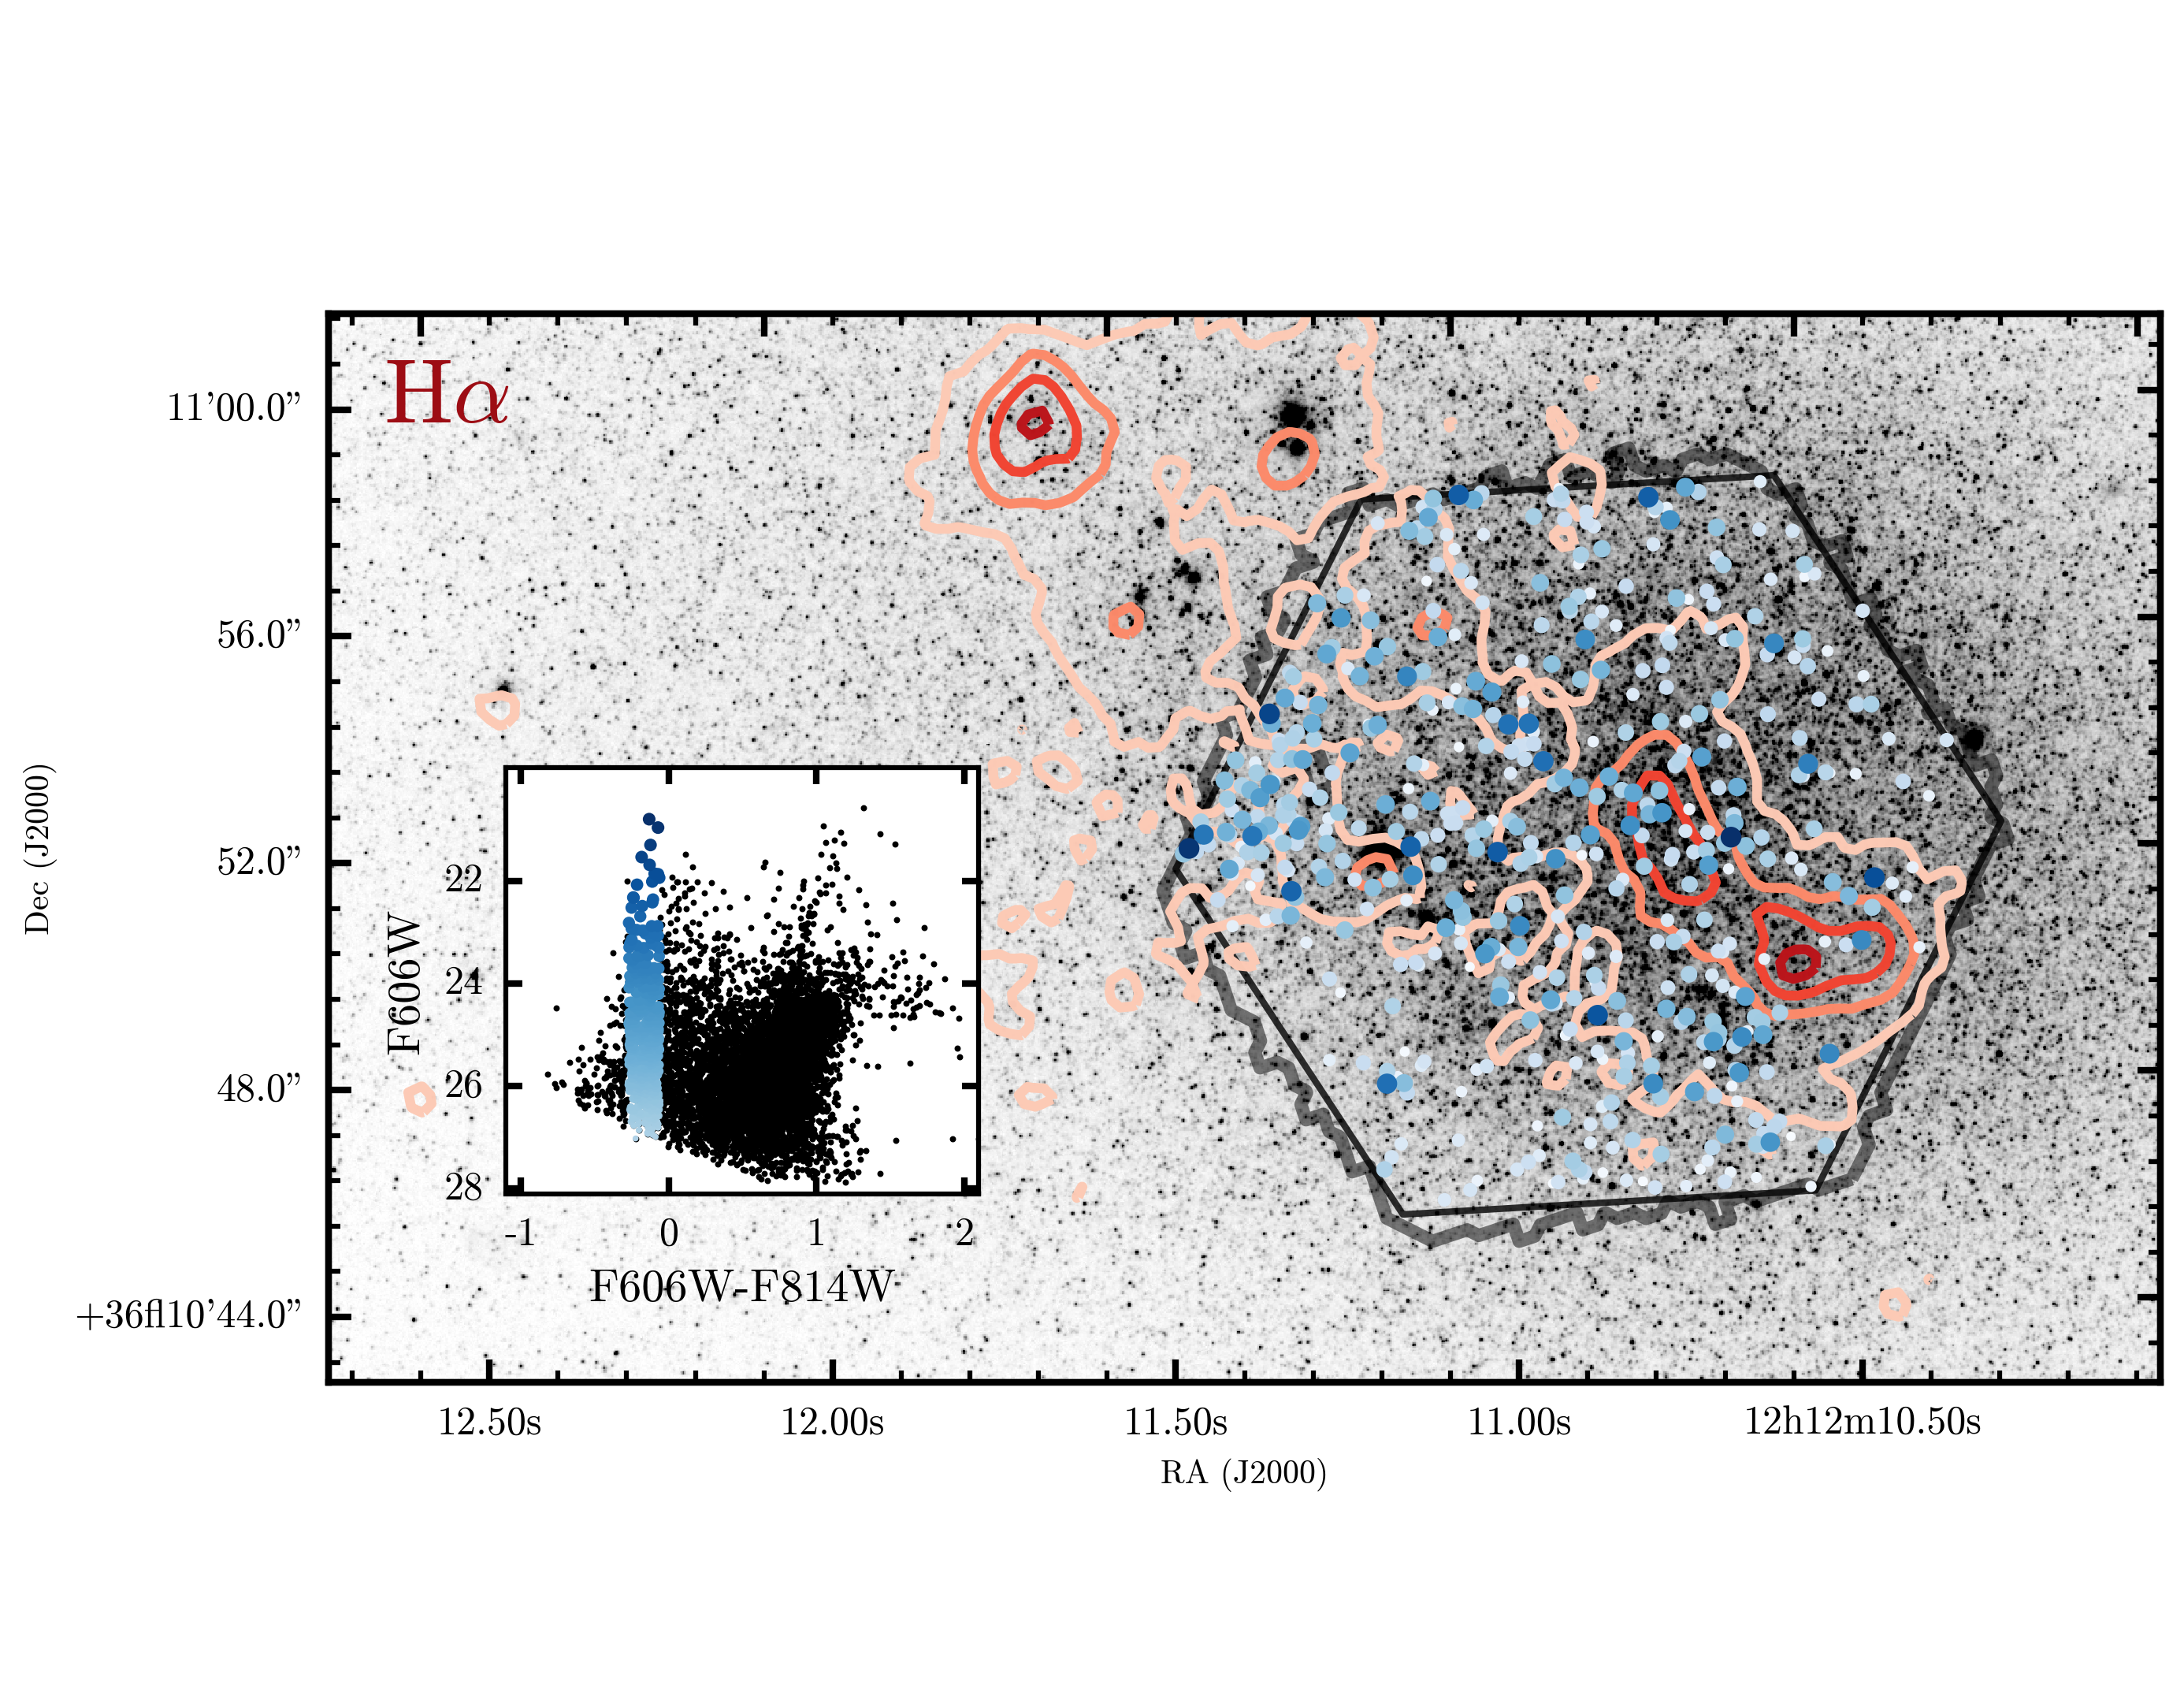
\includegraphics[width=\linewidth]{figs/f1.png}
    \caption{{\sc An aperture-matched comparison of light with HST and MaNGA---} The F606W image of NGC 4163 (greyscale), with the footprint of the MaNGA observations approximated with the black hexagon. \ha contours from the Local Volume Legacy survey are shown in red, with the strongest \ha emission shown in the darkest red lines \citep{Kennicutt+2008}. In the bottom left corner of the figure, we show an inset colour-magnitude diagram for the stars in the hexagon region, F606W-F814W \vs F606W. Main sequence stars are highlighted in blue, where darker blue points represent more luminous main sequence stars. The spatial location of the selected main sequence stars is also shown on the F606W image. Young, hot stars are located throughout the MaNGA observation, with some spatial clustering near known OB associations.}
    \label{fig:FOV}
  \end{center}
\end{figure*}
% actual boundary is weirder though. Do you have an exposure time map for MaNGA showing actual depth accross field after dithering? Hard to see faint MS stars, add MaNGA obs PSF and spaxel size. Leaking edges?
%-------------------------------------------------------

\subsection{HST observations of NGC 4163}\label{sec:data:hst}

NGC 4163 has multi-band archival imaging from HST, analyzed as a part of the ACS Nearby Galaxy Survey Treasury \citep[ANGST;][]{Dalcanton+2009, Dalcanton+2012}. Full details of the survey and photometry can be found in \citet{Dalcanton+2009}.

We use optical photometry (F606W and F814W filters) from the ``{\tt .gst}'' catalogs, which only include stars with the highest quality photometry. The ``{\tt .gst}'' catalogs were compiled following procedures developed by \citet{Dolphin+2000} as described in \citet{Dalcanton+2012}. The stars in the ``{\tt .gst}'' catalog have S/N$ > 4$ in both filters and pass stringent goodness-of-fit cuts. These cuts leave stars with the highest quality photometry but with higher incompleteness in more crowded regions. We then select those stars that fall within the boundary of the MaNGA IFU observation boundaries to create a single catalog of aperture-matched stars.

\textbf{!!! Actually, Dan re-ran the photometry around 7/1/16: }\emph{``The photometry is of the entire ACS field, while the fake stars are just for a region around the MANGA footprint. These are only roughly gst files — I did this by hand and couldn't remember the exact data naming scheme.  It should be self-explanatory, but you'll have to check to make sure you're grabbing the correct columns. I've also already applied quality cuts to the photometry and fake stars.  So all you have to do is grab the data, cut out the RA and DEC region of interest, and run it through MATCH — you don't need to apply any photometric quality cuts.''} \textbf{@Dan: I'm assuming ``roughly gst'' means the files may not have correct naming convention or proper columns, but quality cuts are still those described in Dalcanton+2012? Are there any important details about the new photometry I should include?}

In Fig.~\ref{fig:cmd}, we show two CMDs for NGC 4163. The CMD shown in the left panel includes photometry from the full ACS field of view (${\sim}74,000$ stars), while the right panel shows the photometry extracted from the region mapped to the MaNGA observations (${\sim}7,000$ stars). The arrow shows the direction of 1 magnitude of extinction.

The full-field CMD (left panel of Fig.~\ref{fig:cmd}) shows a well-defined red giant branch (RGB), a well-populated red clump (RC) and main sequence (MS). In the aperture-matched CMD (right panel of Fig.~\ref{fig:cmd}), the MS and RGB are also evident. However, the photometry in the aperture-matched region is significantly shallower than the photometry from the full field, due to higher crowding in the central region of the galaxy. Crowding in regions with high stellar density can strongly affect the photometry, since fewer faint stars will be resolved in a dense field with many bright stars. Faint stars that would otherwise not be detected are biased brighter by blending with neighboring stars.

While the full-field CMD in Fig.~\ref{fig:cmd} has an easily-distinguishable red clump, the aperture-matched CMD is too shallow to reach the depth of the red clump. Unfortunately, the red clump is an important age anchor in the CMD-fitting routine, and the lack of red clump stars introduces significant degeneracies between distance and foreground reddening determinations. To mitigate these effects, we choose to fix the distance and foreground extinction when fitting the CMD with MATCH. We fix the distance modulus to $\dmod = 27.29$ (2.87\,Mpc), based on the TRGB distance determined by \citet{Dalcanton+2009}. We fix the foreground extinction at $\Av=0.06$, which is based on galactic extinction from the \citet{Schlafly+2011} recalibration of the \citet{Schlegel+1998} infrared-based dust map. The map is based on dust emission from COBE/DIRBE and IRAS/ISSA; the recalibration assumes a \citet{Fitzpatrick+1999} reddening law with $R_{\mathrm{v}} = 3.1$ and different source spectrum than \citet{Schlegel+1998}.

%-------------------------------------------------------
% Figure 2: CMDs
%-------------------------------------------------------
\begin{figure*}
  \begin{center}
    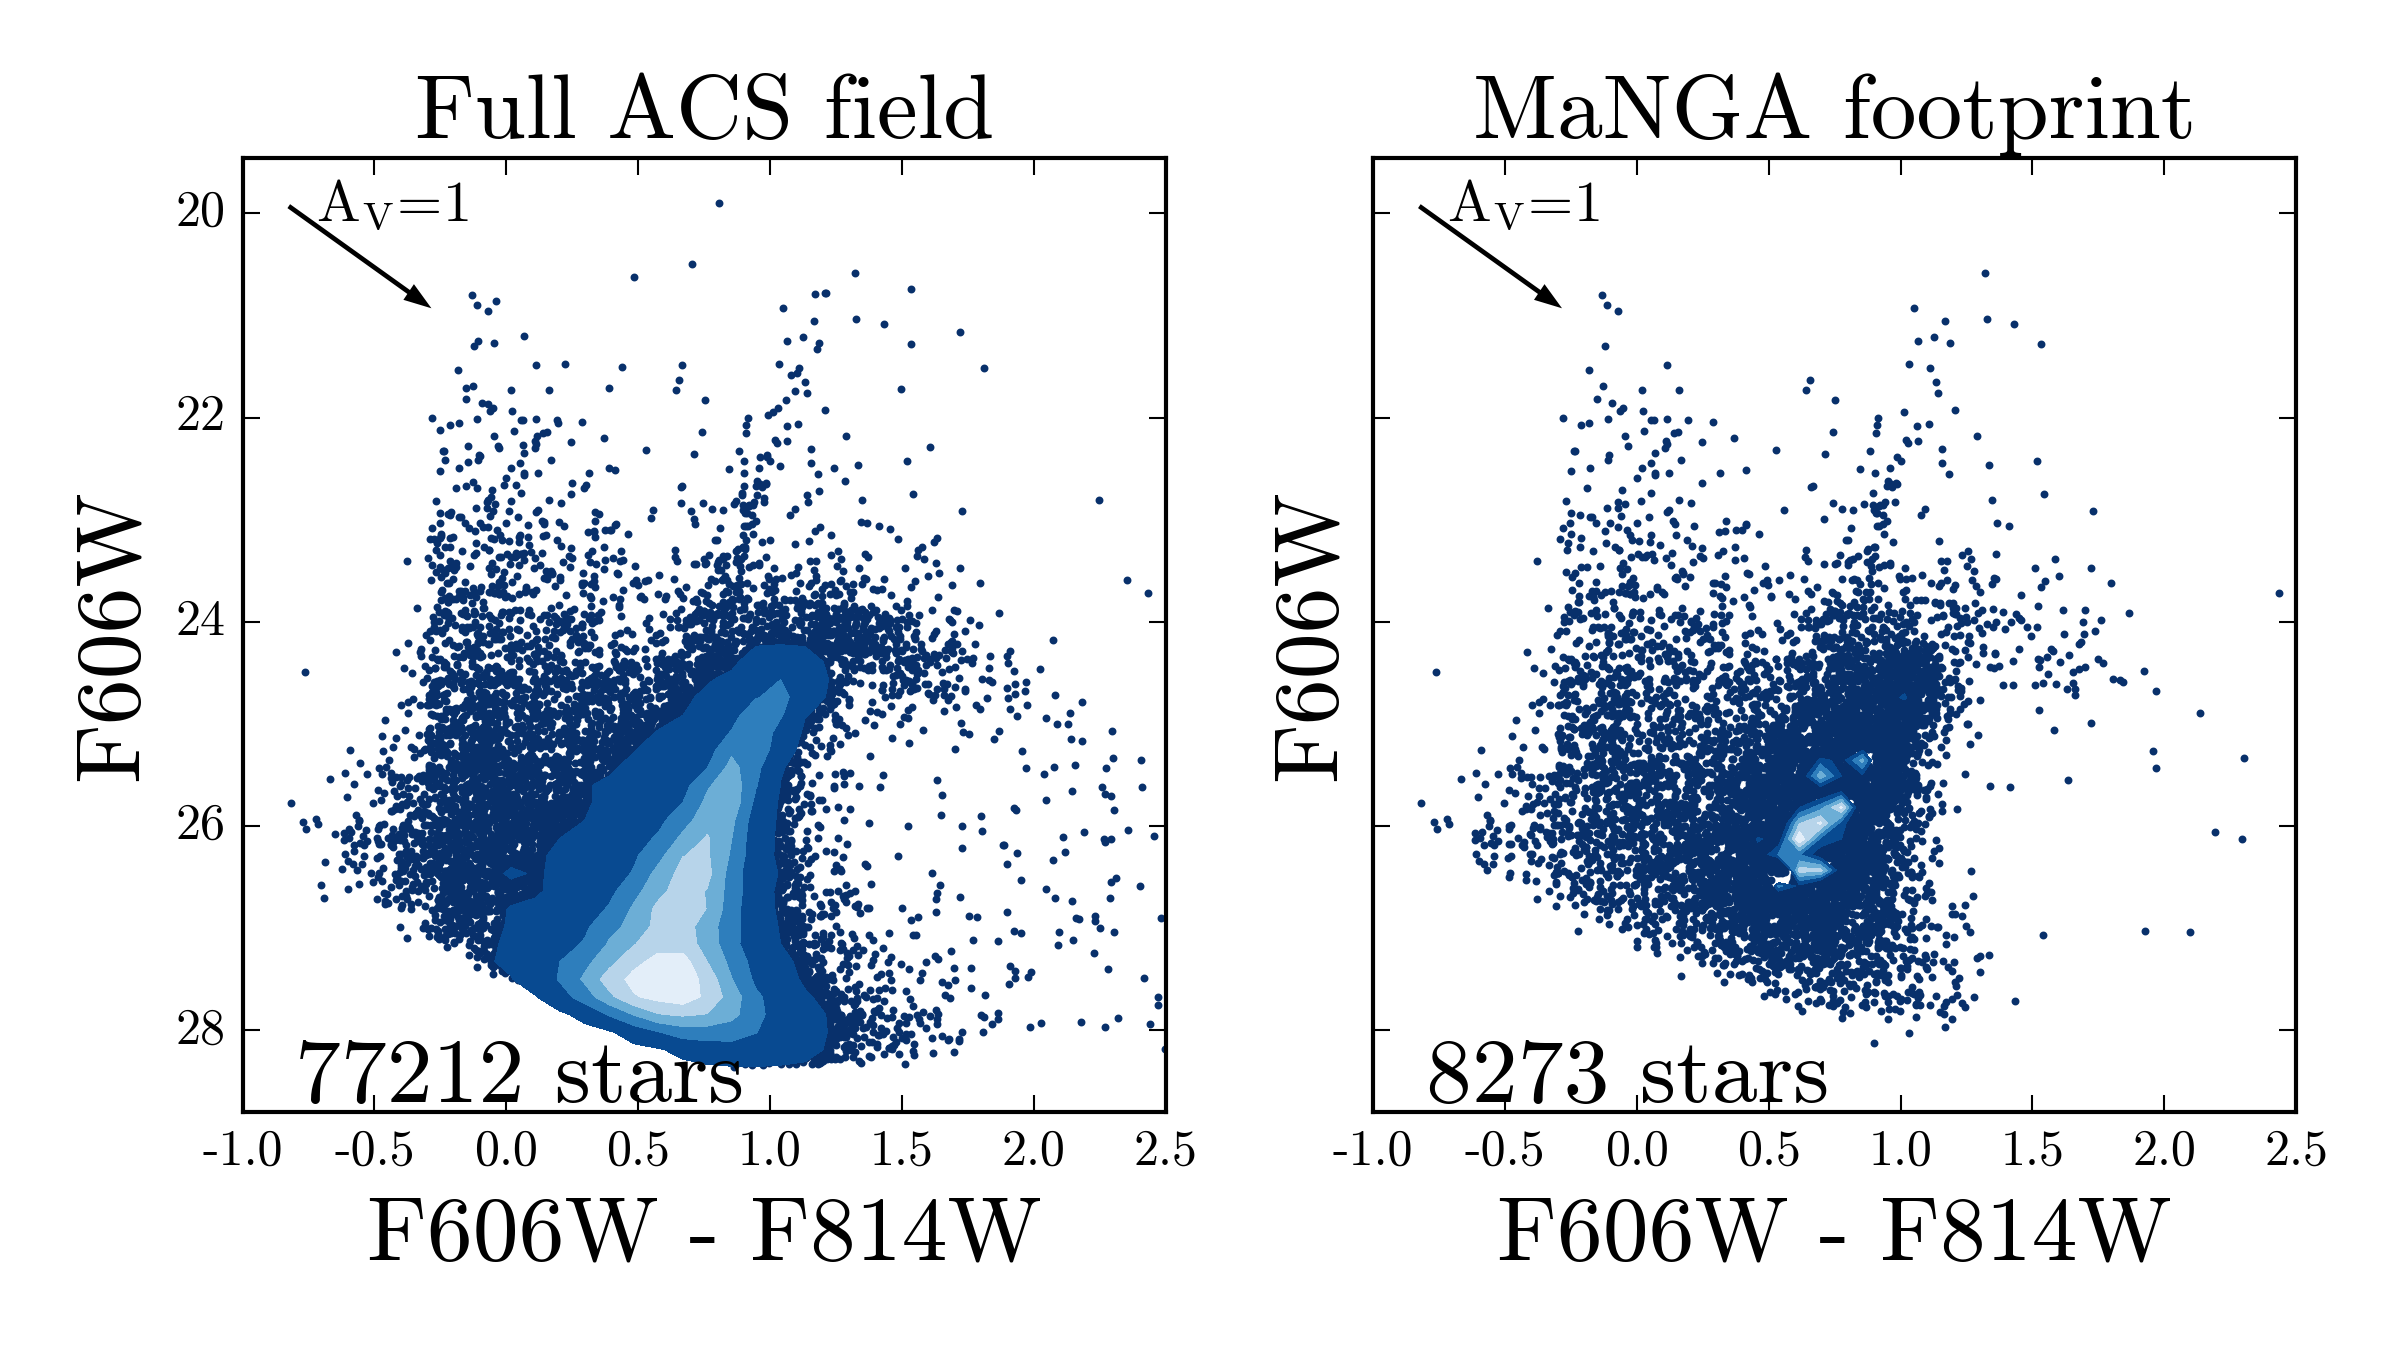
\includegraphics[width=\linewidth]{figs/f2.png}
    \caption{{\sc NGC 4163 color-magnitude diagrams---} \emph{Left:} The CMD for the full ACS field of view, which includes ${\sim}77,000$ stars. \emph{Right: } The CMD of stars extracted from the region mapped to the MaNGA observations, which includes ${\sim}9,000$ stars. The photometry in the aperture-matched region is significantly shallower than the photometry from the full field, due to higher crowding in the central region of the galaxy.}
    \label{fig:cmd}
  \end{center}
\end{figure*}
%-------------------------------------------------------

\subsubsection{Artificial Star tests}

To characterize the photometric completeness and account for observational errors that result from crowding, we preform extensive artificial star tests (ASTs). In these tests, we insert fake stars into each image and rerun the photometry as before. We test for the recovery of these fake stars, and measure the difference between the input and recovered magnitude if the star was detected. The ASTs are used to construct a noise model that accounts for completeness, photometric uncertainties, and color or magnitude biases.

The region covered by the MaNGA observations is significantly more crowded than the full ACS field-of-view. When running MATCH on the CMD from the aperture-matched region, we used a sample of fake stars representative of those found in the crowded central region. In total, we inserted $565,659$ artificial stars individually into the full ACS image. The aperture-matched region contains the results of $65,318$ ASTs.

We show the results from the aperture-matched ASTs in Fig.~\ref{fig:comp}, showing the photometric completeness as a function of magnitude for the F606W filter (left) and the F814W filter (right). In both panels, the red line represents the magnitude at which 80\% of the inserted fake stars are recovered.

%-------------------------------------------------------
% Figure 3: AST 50% completeness
%-------------------------------------------------------
\begin{figure}
  \begin{center}
    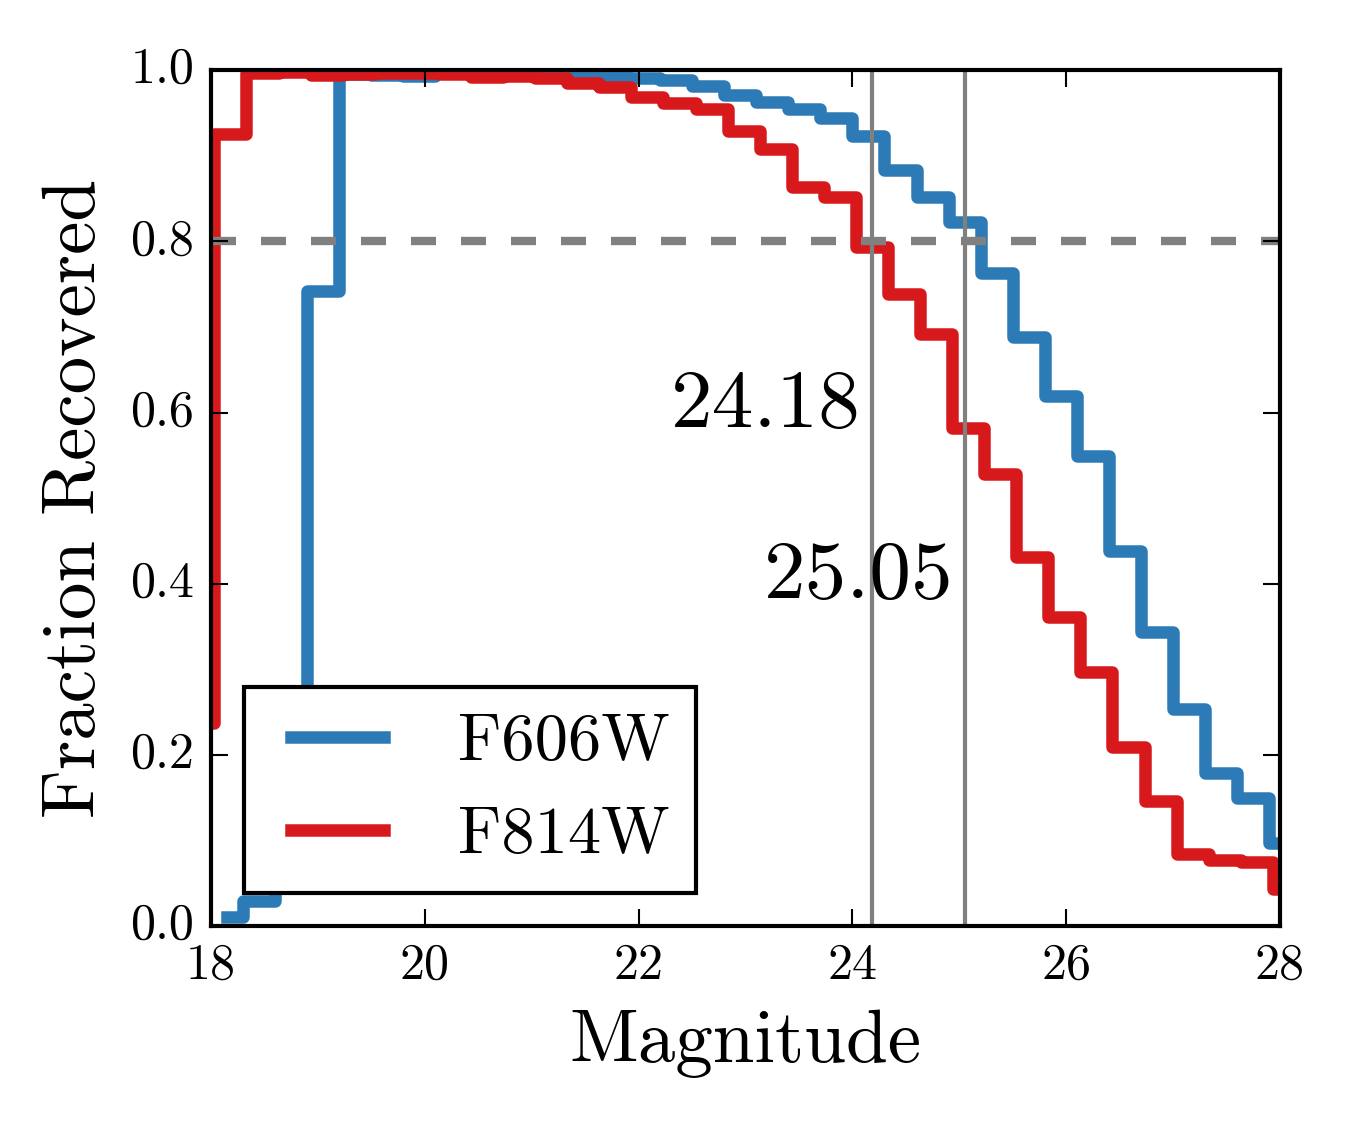
\includegraphics[width=\linewidth]{figs/f3.png}
    \caption{{\sc Photometric completeness for stars in the aperture-matched region---} The 80\% completeness limit for the F606W filter (blue) and the F814W filter (red), computed using fake stars representative of the spatial region mapped to the location of the MaNGA observations.}
    \label{fig:comp}
  \end{center}
\end{figure}
%-------------------------------------------------------


\section{Methods}\label{sec:methods}

Broadly, the procedure for the aperture matched comparison is as follows: We extract HST stellar photometry from the area matched to the MaNGA observation, and fit the CMD of those stars using MATCH \citep{Dolphin+2002} to derive the history of star formation, the chemical evolution history, total stellar mass, and the total and differential extinction. We use the CMD-inferred properties as inputs to the SPS code FSPS \citep{Conroy+2009} to produce a model spectrum, which we compare to the total integrated spectrum observed with MaNGA. Additionally, we use the spectral fitting code \texttt{Prospector} \citep{Johnson+2017} to fit the total integrated spectrum from MaNGA, to compare the SFH determinations from CMD and integrated light techniques. We detail each of these steps below.

\subsection{MATCH input parameters}\label{sec:methods:match}
\begin{deluxetable}{cccc}
\tablecolumns{4}
%\tabletypesize{\scriptsize}
\tablewidth{0pt}
\tablecaption{MATCH parameters}
\tablehead{
    \colhead{$A_{V}$} & %foreground extinction (Schlegel et al. 1998)
    \colhead{$(m-M)_0$} & % distance modulus
    \colhead{$M_{F814W}$ 80\%} &
    \colhead{$M_{F814W}$ 80\%} \\
        \colhead{} & % Av
        \colhead{} & % dmod
        \colhead{Completeness} &
        \colhead{Completeness} \\
            \colhead{(1)} & %Av
            \colhead{(2)} & %dmod
            \colhead{(3)} &
            \colhead{(4)}
      }
\startdata
%0.06 & 27.29 & 26.25 & 25.38 \\
0.06 & 27.29 & 25.05 & 24.18 \\
% A_v   & dmod         & comp  & comp
\enddata
\tablecomments{(1) Foreground extinction \citep{Schlegel+1998}; (2) distance modulus in F814W from \citet{Dalcanton+2009}; (3)  80\% completeness limit ($M_{F606W}$); (4)  80\% completeness limit ($M_{F814W}$).}
\label{tab:matchIN}
\end{deluxetable}
We measure the SFH of NGC 4163 using the maximum likelihood CMD fitting routine, MATCH \citep{Dolphin+2002}. For a set of input parameters (e.g., IMF slope, binary fraction, age bin width, etc.) MATCH constructs synthetic CMDs from SSPs and linearly combines them with a model foreground CMD to form a composite model CMD with a complex SFH. The CMD is convolved with the noise model generated from the ASTs. The model CMD is compared with the observed CMD using a Poisson likelihood statistic. The process is repeated for various weights on the SSPs until the likelihood function is maximized. The synthetic CMD that best matches the observed CMD is deemed to have the most likely SFH that produced the data. Full details are given in \citet{Dolphin+2002}.

In this work we have adopted the following parameters for the SFH solutions, summarized in Table~\ref{tab:matchIN}. As discussed in \S\ref{sec:data:hst}, we assume a fixed distance modulus of $\dmod = 27.29$. We assume a \citet{Chabrier+2003} IMF, and a binary fraction of 0.35, with the mass of the secondary drawn from a uniform distribution of mass ratios. We use the C3K theoretical spectral library and the MIST stellar evolution models from \citet{Choi+2016, Dotter+2016}, with mass limits from 0.1 to 300\Msun. We used the combination of MIST and C3K so that the same isochrones and stellar library are used to fit the CMD \emph{and} to generate the synthetic spectrum in FSPS. We discuss the use of alternative isochrones and stellar spectral libraries in \ref{sec:discussion}.

\paragraph{SFH specifications}
Due to the shallow photometric depth in the aperture-matched region, we derive the SFHs using only the optical data from the F606W and F814W filters, which provide the deepest CMDs. We designated the faint photometric limit to be equal to the 80\% completeness limit in each filter (see Table~\ref{tab:matchIN}) as determined by the artificial star tests run for each galaxy. %We discuss the use of more conservative photometric limits (at the 80\% completeness limit) in \ref{sec:discussion}.

We solve for the SFH in 68 time bins covering a range in log time from 6.6 to 10.15 years, spaced by 0.1 dex between 6.6 and 8.7, and by 0.05 dex between 8.7 and 10.15. We are limited by the depth of the data, which does not reach the red clump, and so we constrain the metallicity to only increase with time. We limit the oldest time bins to have [M/H] between -2.5 and -1.0 and the youngest time bin to have [M/H] between -1.0 and 0.0. Within each time bin, however, we permitted a $1\sigma$ metallicity dispersion of 0.15 dex, which provides the flexibility to capture potential metallicity spreads at each age.

\paragraph{Dust}
MATCH allows two free parameters to describe the dust distribution: a foreground extinction, \Av, and a differential extinction, \dAv, which describes the spread in extinction values for the stars in the region. We use an age-dependent differential extinction model for stars with ages $<100$\Myr, as specified in \citet{Dolphin+2003}. In this model, stars with ages between 100 and 40\Myr have a linearly increasing maximum differential extinction, from \dAv$= 0.0$ at 100\Myr to \dAv(max) mag at 40\Myr. Stars with ages below $40$\Myr have a maximum extinction of \dAv(max) mag in \Av. This model provides optimal fits to the young stellar populations in a variety of nearby dwarf galaxies \citep[e.g.,][]{Dolphin+2003, Skillman+2003, Weisz+2011}, and is necessary to reproduce the observed integrated blue-optical and ultraviolet light of dwarf galaxies in the Local Volume \citep{Johnson+2013}. As discussed in \S\ref{sec:data:hst}, we assume that the foreground extinction is fixed at \Av$=0.06$. However, we allow \dAv to vary between 0.0 and 1.0.

\subsection{Generating model spectrum with FSPS using the CMD-inferred SFH}\label{sec:methods:fsps}

In this section, we describe the process for generating the model spectrum using the CMD-derived SFH. 

For stellar population synthesis, we use the Flexible Stellar Population Synthesis package \citep[\FSPS;][]{Conroy+2009, Conroy+2010} via the Python interface, \pFSPS \citep{pythonFSPSdfm}. We note that the isochrone set, spectral library, and IMF used to construct the model spectrum are identical to those used within MATCH for CMD fitting, to make the most robust comparison.

Specifically, we use the MESA Isochrones \& Stellar Tracks \citep[MIST;][]{Dotter+2016, Choi+2016}, single-star stellar evolutionary models which include the effect of stellar rotation. The evolutionary tracks are computed using the publicly available stellar evolution package Modules for Experiments in Stellar Astrophysics \citep[MESA v7503;][]{Paxton+2011,Paxton+2013, Paxton+2015}. We combine the MIST tracks with a high resolution theoretical spectral library (C3K; Conroy, Kurucz, Cargile, Castelli, \emph{in prep}) based on Kurucz stellar atmosphere and spectral synthesis routines \citep[ATLAS12 and SYNTHE,][]{Kurucz+2005}. For all other SPS parameters, we use the default parameters in \FSPS\footnote{GitHub commit hash \texttt{4e1b3f5}}.

\paragraph{SFH and age-metallicity relation}
To generate our model spectrum, we use three outputs from MATCH: (1) the total stellar mass formed in the area observed, (2) the fraction of the total stellar mass formed within each time interval, and (3) the metallicity of the stars formed in each time interval. We refer to the combination of (1) and (2) as the CMD-based SFH, and (3) as the CMD-based chemical evolution history, or CEH.

We first resample the MATCH SFH and CEH onto the more finely sampled native time resolution of the isochrones, ensuring that the mass integrated over the MATCH time interval is preserved in the resampled SFH. This process implicitly assumes a constant SFH throughout the duration of each time bin. At each time step, we select the SSP with metallicity determined by the CEH, and generate a spectrum. This process leaves us with an array of SSP spectra at each age.

We redden each model spectrum using both the foreground extinction \Av, and the differential extinction \dAv returned by MATCH. We use the same age-dependent differential extinction model used during the CMD-fitting process, with the best-fit value of \dAv(max) to scale the maximum differential extinction.

We sum the array of SSP spectra, weighting each spectrum by the fraction of mass formed at that age, as determined from the SFH. The result is a single spectrum, reflecting the mass-weighted ages and chemical compositions from the CMD-derived SFH and CEH.

To compare the synthesized spectrum with the total observed spectrum from MaNGA, we use the distance modulus assumed in \S\ref{sec:methods:match} to scale the absolute flux level of the model spectrum, which we convert to $10^{-17}$erg/s/cm$^2$/\ang, the units of the observed spectrum.

\paragraph{Spectral Resolution}
The C3K library has R=10,000 between 1500\ang and 10,000\ang. The MaNGA observations typically have spectral resolution $R\sim2000$, so we smooth the model spectrum with a wavelength dependent line-spread function. We use the wavelength array, $\lambda_{\mathrm{MaNGA}}$, from the MaNGA datacube (de-redshifted using the redshift from the Data Analysis Pipeline $z=0.000547$) and the associated spectral resolution array, $R_{\mathrm{MaNGA}}$ (i.e., $\lambda$/d$\lambda$) which provides the median spectral resolution as a function of wavelength for the fibers in the IFU. To compute $\sigma_{\mathrm{MaNGA}}$, the dispersion in \ang, we divide the wavelength array, $\lambda_{\mathrm{MaNGA}}$, by the spectral resolution array, $R_{\mathrm{MaNGA}}$. We then divide $\sigma_{\mathrm{MaNGA}}$ by 2.355 to convert to FWHM, giving the wavelength-dependent line-spread function {\tt lsf}$_{\mathrm{MaNGA}}$. We interpolate {\tt lsf}$_{\mathrm{MaNGA}}$ onto the model wavelength array, and then smooth the model spectrum using {\tt lsf}$_{\mathrm{MaNGA}}$ with a FFT convolution. We note that this process does not correct for the template resolution of the spectral library. However, this should only present an issue if we are interested in making detailed kinematic comparisons. We thus choose to omit the correction.
 
\paragraph{Nebular Emission}
We generate two model spectra: one that includes nebular line and continuum emission, and one that does not. For the spectrum that includes nebular emission, we use the \Cloudy nebular model implemented within \FSPS, \CloudyFSPS \citep{cloudyFSPSv1}, which scales the nebular emission with the ionizing photon flux from the stellar spectrum. The full details of the nebular model can be found in \citet{Byler+2017}.

We emphasize that MATCH is not sensitive to stellar populations with ages below 4\Myr, the youngest Padova SSP included in MATCH. Thus, we cannot provide any constraints on the nebular emission properties, and our assessment of the nebular emission will remain qualitative. The gas phase metallicity is scaled to match the present-day stellar metallicity, inferred from the CMD. We assume a modest value for the ionization parameter, \logU, (\logUeq{-4}), since the emission morphology is quite diffuse, and several low ionization lines are observed (e.g., \sii).

\subsection{Spectral fitting on the total MaNGA spectrum with \texttt{Prospector}} \label{sec:methods:pros}

We take a complementary approach to testing the consistency between SFHs derived from CMD modeling and from SPS modeling. The spectrum reconstruction method described in the previous Section is detailed and robust, but is far more complex than the models in most state-of-the-art spectral fitting codes. We use \texttt{Prospector}\footnote{https://github.com/bd-j/prospector; GitHub commit hash b0ea36e} \citep{Johnson+2017, Leja+2017}, a Bayesian spectral fitting code, to infer the SFH of the area of NGC 4163 covered by the MaNGA observations described in \S\ref{sec:data:manga} above. A key strength of this software is its flexible SFH parameterization: we can infer the star formation rate in age bins analogous to the \texttt{MATCH} time bins (though with coarser time resolution), rather than imposing a smoothly varying analytic form on the model SFH. We describe the parameters and assumptions in our modeling, then compare our inferred SFH to the ``gold standard'' SFH from the CMD modeling (presented in \S\ref{sec:results:match} below). 

\subsubsection{Details of the \texttt{Prospector} Model}

The \texttt{Prospector} code calculates the posterior distribution of stellar population parameters, given the observed galaxy spectrum and priors on the free model parameters. The mock spectra are generated using FSPS, accessed via the \texttt{python-fsps} wrapper. We sample the parameters used to generate model spectra using a nested sampling code, \texttt{nestle}\footnote{https://github.com/kbarbary/nestle; GitHub commit hash 1b47f3f}, to ensure that the likelihood surface is fully explored \citep[e.g.,][]{shaw07, feroz09}. 

For our \texttt{Prospector} model, we adopt a \citet{kroupa01} IMF, the empirical MILES spectral library \citep{sanchez-blazquez06}, and the Padova isochrone set \citep{girardi00, marigo08}, supplemented with the Geneva isochrones for high-mass stars \citep{schaller92, meynet00}. These choices differ from those made in the MATCH modeling and synthetic spectrum generation described in \S\ref{sec:methods:fsps} and \ref{sec:methods:match} above, but result in a factor of several decrease in computation time and do not substantially affect either the fit quality or the inferred galaxy parameters. We impose the same distance modulus and foreground $A_V$ as in the MATCH modeling (see \S\ref{sec:methods:match}). 

In what follows, we describe each of the free parameters in the model and the priors adopted for each, as summarized in Table~\ref{tab:prospector_params}.

\textit{Star Formation History} --  We use a flexible, ``nonparametric'' SFH model that does not impose a smooth, analytic form on the SFH. Rather, the model determines the average SFR in seven age bins with the following age limits: 0--10 Myr; 10--30 Myr; 30--100 Myr; 100--300 Myr; 300 Myr--1 Gyr; 1--3 Gyr; 3--14.1 Gyr. These bins are chosen to be equally spaced in logarithmic time, except for the oldest and youngest bins, for which the optical spectrum has limited constraining power.

Naively, one would expect the model to fit the stellar mass formed (or the average SFR) in each age bin. However, \citet{leja18} showed that uniform priors on logarithmic $M_\star^\mathrm{formed}$ in each age bin are not well-behaved. Instead, we adopt the method of \citet{leja17}, who fit the shape and normalization of the SFH separately. Our \texttt{Prospector} model fits the ``SFR fractions'' $x_n$ in each age bin, defined as:

\begin{equation}
m_n = \frac{t_n x_n}{\sum_N t_n x_n},
\end{equation}
where $N=7$ is the number of age bins, $t_n$ is the width of each bin, and $m_n$ is the fraction of stellar mass formed in each bin. It is helpful to think of the quantities $x_n$ as the mass fraction formed in each bin, normalized to the width of that time bin. The SFH parameters are subject to the constraint that $\sum_N x_n = 1$, since all stellar mass must have formed during one of the age bins. For $N=7$ bins, we have six free parameters describing the $x_n$, and another free parameter describing the normalization of the SFH, i.e., the total stellar mass formed. We adopt a Dirichlet prior on the SFH $x_n$ \citep[see][for details]{leja17, leja18}, and a uniform prior on the stellar mass: $1.0 < \log{(M_\star^\mathrm{formed}/M_\odot)} < 14.0$.

\textit{Dust} -- The foreground dust extinction is fixed to $A_V=0.06$ and is applied to stars formed in all age bins. However, as described in \S\ref{sec:methods:match} above, young stars are embedded in dust and experience more dust attenuation. \texttt{Prospector} does not have a model analogous to the differential dust extinction implemented in MATCH. We therefore include two free parameters describing the dust attenuation applied to only young stars ($\leq 100$ Myr), in addition to the foreground dust screen. The optical depth, $\tau_V^\mathrm{young}$, and slope of the power-law attenuation curve, $\alpha^\mathrm{young}$, are both free parameters so that the model is flexible enough to approximate the net effect of the differential extinction on young stellar populations.

\textit{Metallicity} -- The stellar metallicity is a free parameter, with a uniform prior distribution between $-2.0 < \log{(Z/Z_\odot)} < 0.2$. 

We fit this \texttt{Prospector} model to the total spectrum of the MaNGA footprint, described in \S\ref{sec:data:manga} above. We mask emission lines in our fitting, but use the \citet{Byler+2017} nebular continuum model to properly account for the contribution of \hii regions to the optical continuum. We assume that the gas-phase metallicity is equal to the stellar metallicity and adopt an ionization parameter of $\log(U) = -4$. We restrict the fit to $4000 < \lambda < 7000 \mathrm{\AA}$ to avoid dense emission lines in the blue and sky background issues in the red. Finally, we inflate the uncertainties on the observed spectrum to achieve a median signal-to-noise of 10 to ensure complete exploration of the parameter space, accounting for the systematic uncertainty inherent in the adopted isochrones, stellar library, and model assumptions.

%%%%% KEEPING THE TABLE AT THE END FOR NOW %%%%%

\begin{table*}
\caption{Free parameters in the \texttt{Prospector} model.} 
\label{tab:prospector_params}
\begin{center}
\begin{tabular}{lc}
\hline \hline
Parameter & Prior \\
\hline
SFH ``SFR fractions'' & Dirichlet prior: $0 < x_n < 1$, $\sum_n x_n = 1$\\
Stellar Mass & $1.0 < \log{(M_\star / M_\odot)} < 14.0$ \\
Metallicity & $-2.0 < \log{(Z/Z_\odot)} < 0.2$ \\
Dust Optical Depth & $0.0 < \tau_V^\mathrm{young} < 1.65$ \\
Dust Attenuation Law Slope & $-3.0 < \alpha^\mathrm{young} < -0.3$\\
\hline
\end{tabular}
\end{center}
\tablecomments{``SFR fractions'' $x_n$ are the fraction of stellar mass formed in each age bin, normalized to the bin width. All other priors are uniform distributions.}
\end{table*}


% ================================================================
\section{Results}\label{sec:results}

\subsection{MATCH results}\label{sec:results:match}
\paragraph{The best fit model CMD}
In Fig.~\ref{fig:matchCMD} we show the results of the CMD-fitting process for NGC 4163. We show Hess diagrams (a 2D density plot of the CMD) for the observed data (a), the best fit model (b), the total residual difference between model and data (c) and the residual significance (d). Overall, we find that the model reproduces the observed CMD reasonably well. The best fit model contains an RGB, SGB, and MS that are well matched to the observations in terms of density of stars, luminosities/colors, and width of features.

Examining the residual significance CMD, i.e., the difference between the data and the model weighted by the variance (the lower right panel of Fig.~\ref{fig:matchCMD}), we can see that the fit is not perfect. In particular, the area between the young stars on the main sequence and the blue helium-burning stars (which bracket F606W-F814W$\,{\sim}\,0$) appears to be too cleanly separated in the model. This discrepancy could indicate that the young stars in the observed CMD are affected by more differential extinction than accounted for in MATCH. However, there are few coherent structures visible in the residual significance Hess diagram (panel (d) of Fig.~\ref{fig:matchCMD}), and even the most discrepant regions are fit within $\pm 5\sigma$, as indicated by the black or white pixels. As such, the perception of difference is not obviously statistically significant.

The best-fit maximum differential extinction for the young populations is $\dAv = 0.5$ mag, which is typical of other local star forming dwarf galaxies \citep{Weisz+2011}. However, the aperture-matched region shows clear spatial variations in the young stellar populations (e.g., Fig.~\ref{fig:FOV}), and it is likely that there are also significant spatial variations in differential extinction. Regions where the differential extinction differs significantly from the best-fit value introduce additional uncertainties associated with the youngest time bin fit by MATCH. %We further discuss the sensitivity to variations in differential extinction in \S\ref{sec:discussion:dav}.

%-------------------------------------------------------
% Figure 4: Hess diagrams and residuals
%-------------------------------------------------------
\begin{figure}
  \begin{center}
    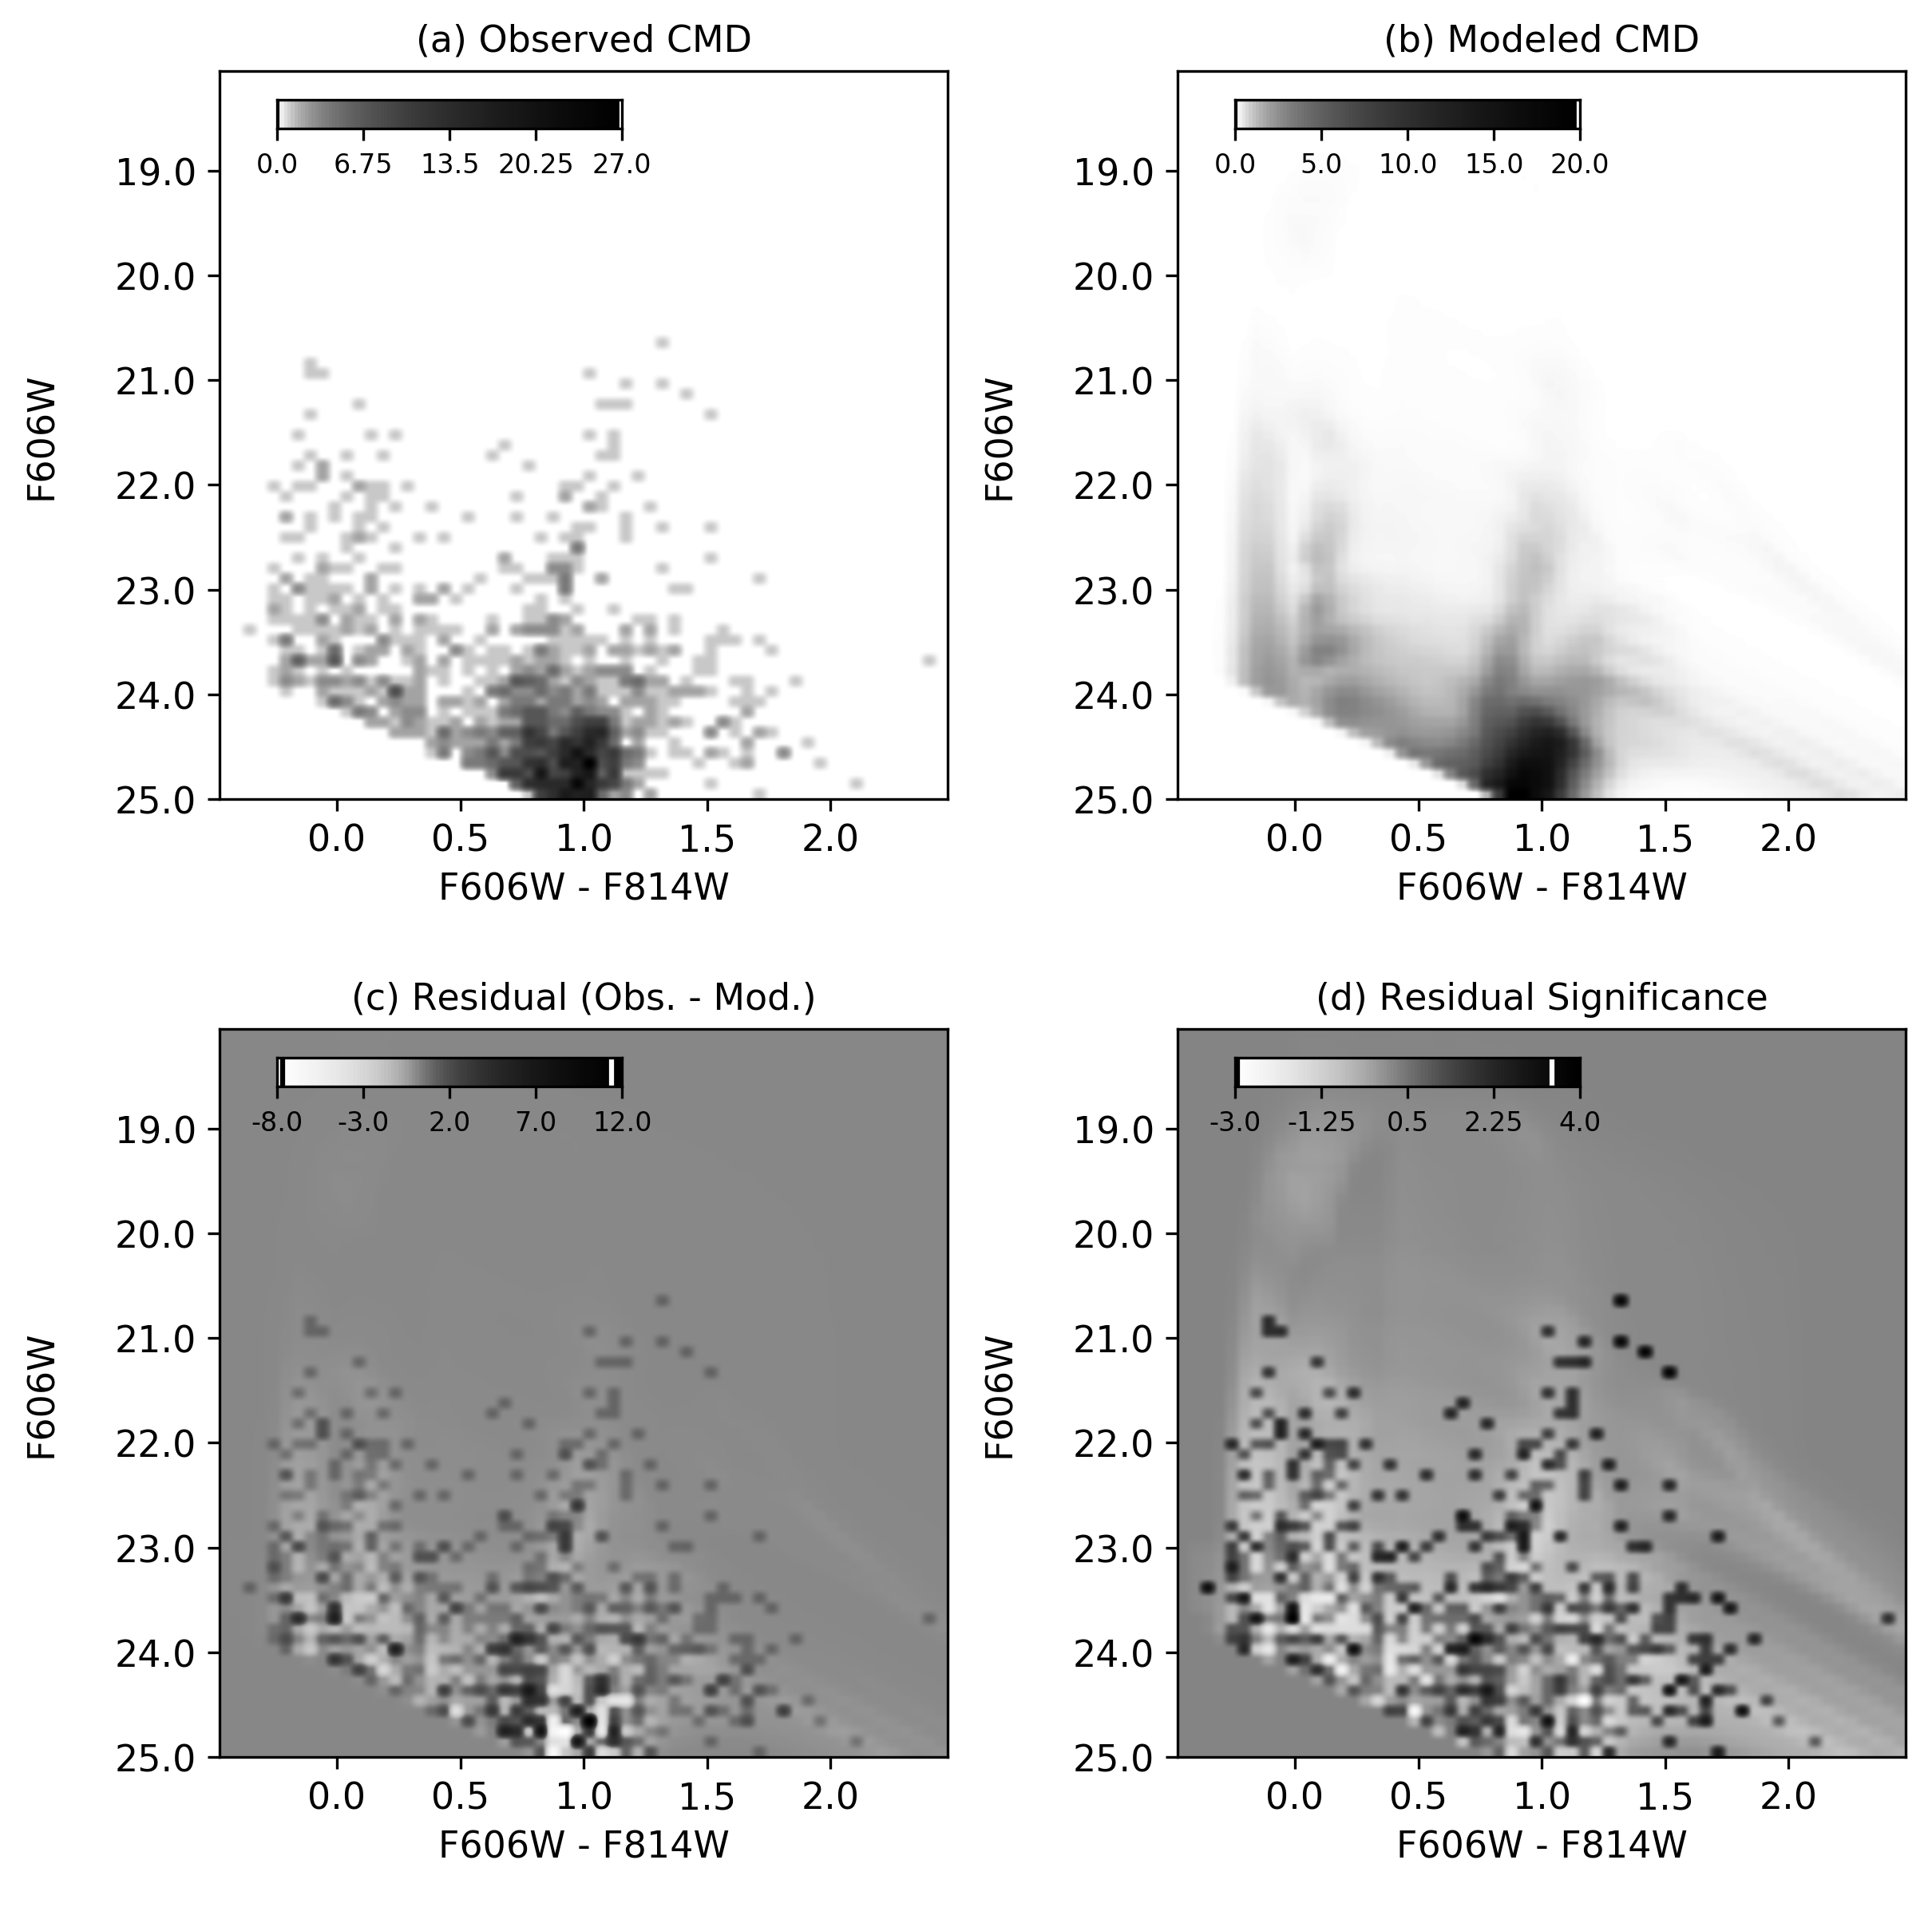
\includegraphics[width=\linewidth]{figs/f4.png}
    \caption{{\sc The best-fit model from CMD-fitting with MATCH---} (a) The observed Hess diagram; (b) the best fit model Hess diagram; (c) residual Hess diagram; (d) residual significance Hess diagram. i.e., the difference between model and data weighted by the variance. In panels (a), (b) and (c), the greyscale reflects the number of stars. In panel (d), the greyscale reflects the significance of each pixel in the residual relative to the standard deviation of a Poisson distribution. Overall, the model reproduces the observed Hess diagram reasonably well, demonstrated in the lack of coherent structure in panel (d).}
    \label{fig:matchCMD}
  \end{center}
\end{figure}
%-------------------------------------------------------
\paragraph{The best-fit star formation history}

In Fig.~\ref{fig:matchSFH}, we show the best fit SFHs for NGC 4163. In the left panel, we show the best fit absolute SFH, or the SFR as a function of time. In the right panel, we show the cumulative SFH, or the fraction of total stellar mass formed prior to or during a given time bin. In both panels, the results for the aperture-matched CMD are shown in blue and the results for the full-field CMD are shown in black (\todo{full field not included yet}). The error bars and error envelopes represent the 16$^{\mathrm{th}}$ and 84$^{\mathrm{th}}$ percentile for the distribution of SFHs computed via the Monte Carlo process described in \S\ref{sec:methods:match}.

The global SFH (as measured from the full-field photometry) and the central, aperture-matched region show similar overall behavior, with a substantial old stellar population (${\sim}50$\% of the total mass) underlying more recent star formation. There is a decline in SFR over the last 100\Myr, with a burst of SF within the last 10\Myr. The aperture-matched region shows a larger fraction of total mass formed in the recent burst of SF, which is expected, considering that the MaNGA observations covered the central part of the galaxy, including several OB associations.

%-------------------------------------------------------
% Figure 5: SFH
%The best fit SFH for NGC 4163, including the region matched to the MaNGA observations (blue) and the full ACS field of view (black).
%-------------------------------------------------------
\begin{figure*}
  \begin{center}
    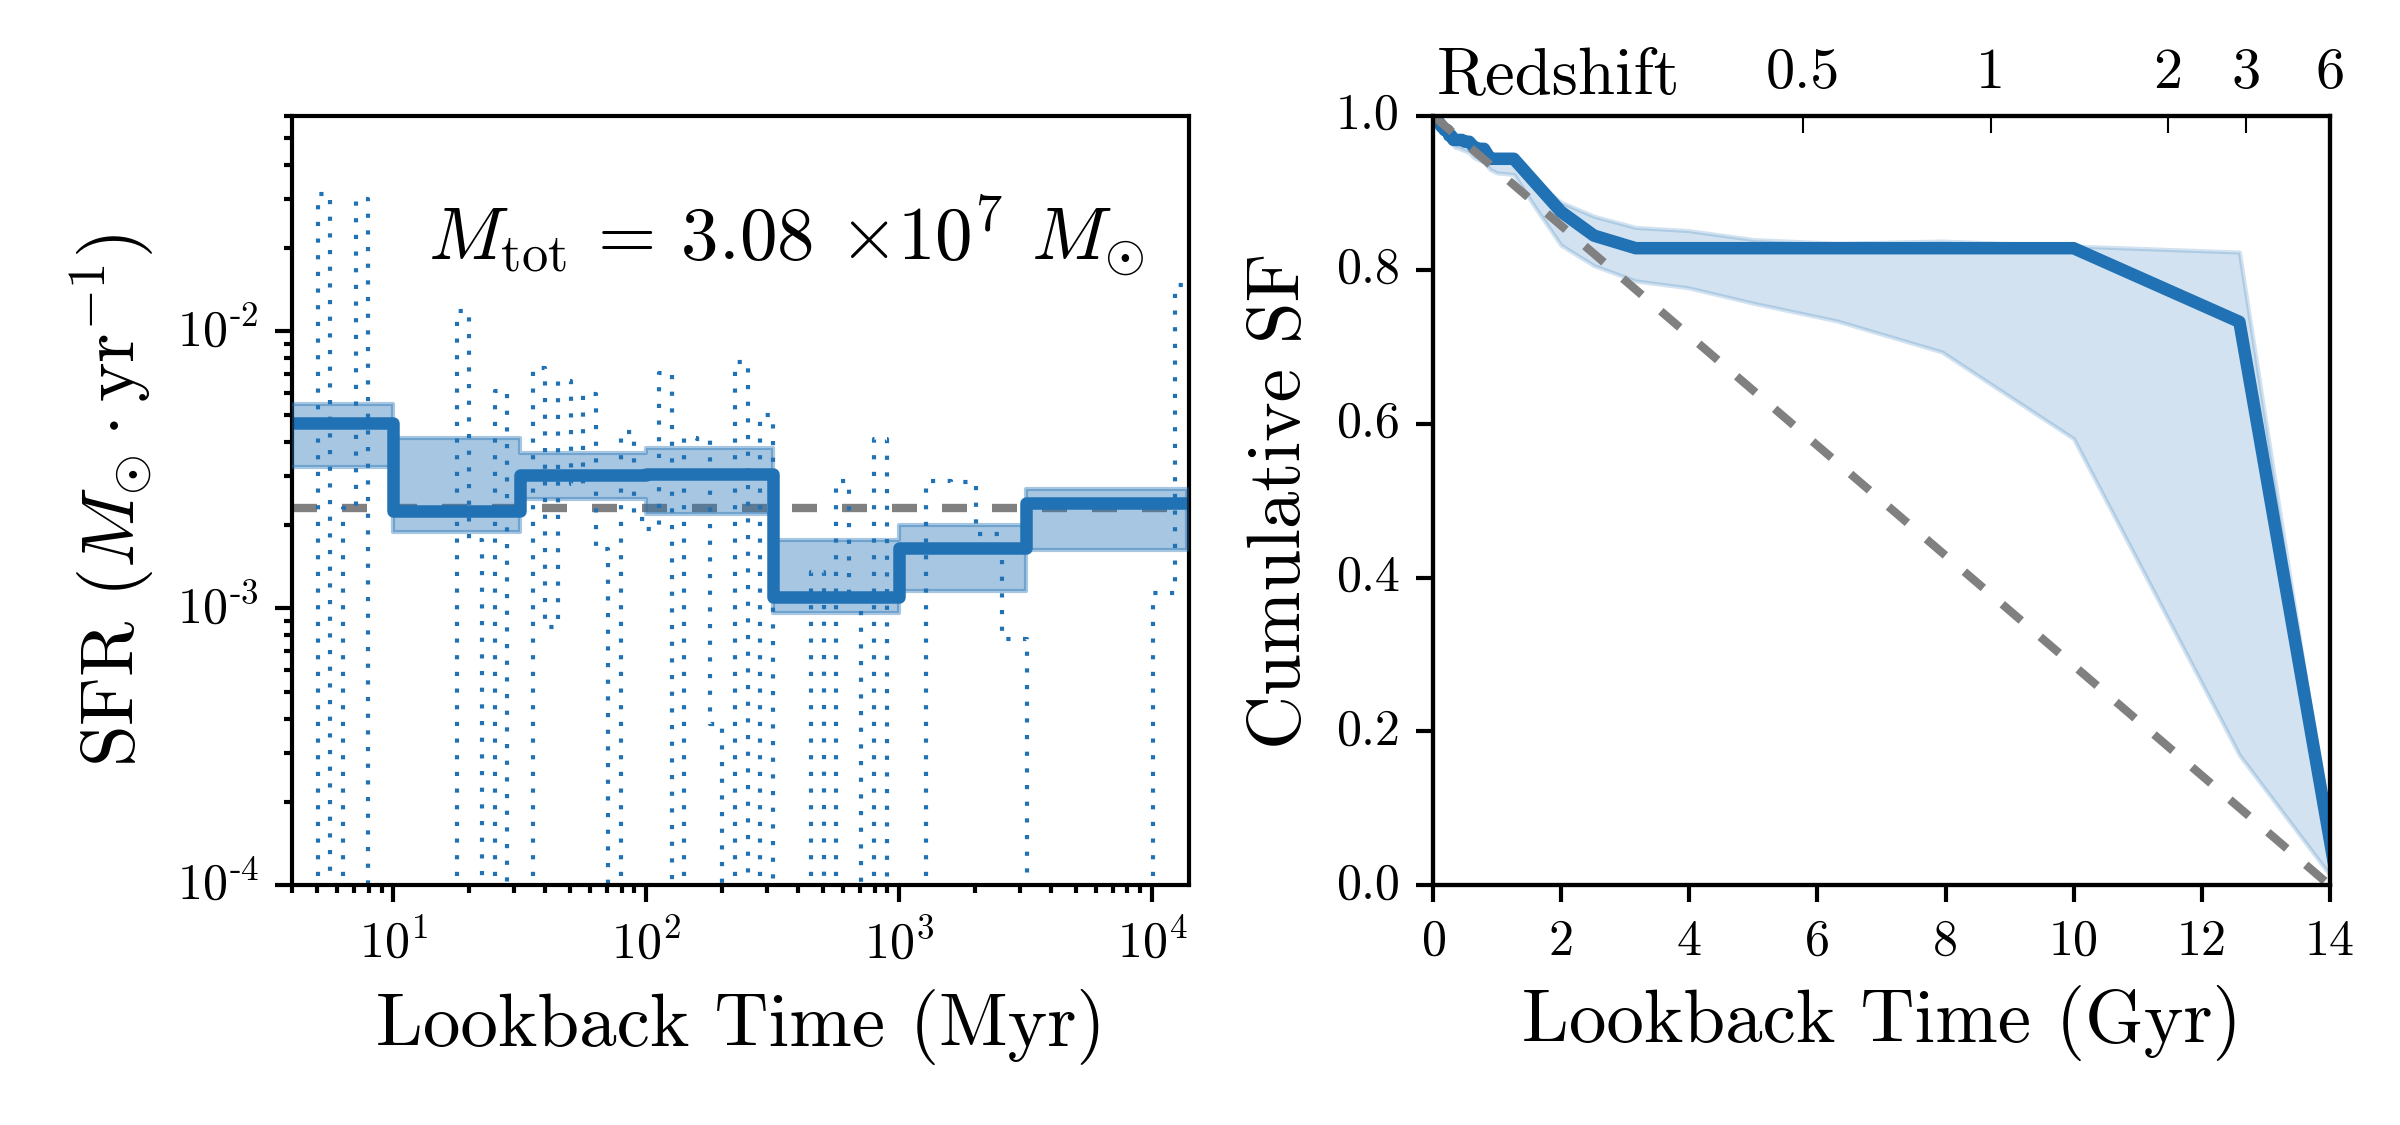
\includegraphics[width=\linewidth]{figs/f5.png}
    \caption{{\sc The best-fit SFH from CMD-fitting---} The left panel shows the absolute SFH (i.e., the SFR(t)), while the right panel shows the cumulative SFH (i.e., the fraction of total stellar mass formed prior to or during a given time bin. The SFH at the native MATCH resolution is shown in the left panel with the blue dotted line. In both panels, the error envelope represents the 16$^{\mathrm{th}}$ and 84$^{\mathrm{th}}$ percentile for the distribution of SFHs computed via the Monte Carlo process. In the left panel, the grey dashed line represents the lifetime-averaged SFR; in the right panel it shows a slope of unity, i.e., a constant SFR.}
    \label{fig:matchSFH}
  \end{center}
\end{figure*}
%-------------------------------------------------------
\begin{deluxetable}{cccc}
\tablecolumns{3}
%\tabletypesize{\scriptsize}
\tablewidth{0pt}
\tablecaption{best-fit parameters from MATCH}\label{tab:matchBF}
\tablehead{
    \colhead{$dA_{V}$} & 
    \colhead{[M/H]$_{\rm today}$} & 
    \colhead{$M_{\star}$}
      }
\startdata
0.5 & -0.6 & $3\times10^{7}\Msun$ \\
% A_v   & dmod         & comp  & comp
\enddata
\end{deluxetable}
\paragraph{Other best-fit properties from MATCH}

The full results from the best-fit model from MATCH are given in Table~\ref{tab:matchBF}. The present-day metallicity determined from MATCH is [M/H] = -0.6, which is consistent with other metallicity estimates from CMD-fitting \citep[e.g.,][]{Rosenfield+2016}. This present-day stellar metallicity translates to an oxygen abundance of $12+\log_{10}(\mathrm{O}/\mathrm{H}) = 8.09$, assuming solar-scaled abundances and a solar oxygen abundance of $12+\log_{10}(\mathrm{O}/\mathrm{H}) = 8.69$, larger than the direct-temperature estimate of $12+\log_{10}(\mathrm{O}/\mathrm{H}) = 7.56$ from \citet{Berg+2012}.

%The aperture-matched region contains $3\times10^7\Msun$ of stars. As discussed in \S\ref{sec:data:hst}, the shallow photometry in the central region of NGC 4163 and the likelihood of spatial variations in differential extinction and completeness limit the ability of MATCH in determining total stellar mass.


\subsection{CMD-inferred model spectrum}\label{sec:results:fsps}

In Fig.~\ref{fig:fullSpec}, we compare the total summed MaNGA spectrum (black) to the model spectrum generated from the CMD-inferred properties (blue; described in \S\ref{sec:methods:fsps}) between 3800 and 8800\ang. The bottom panel shows the percent residual difference between the model and observed spectrum. 

We note that the model spectrum is $\sim30$\% brighter than the observed spectrum. The mismatch in total flux between model and data is likely due to the shallow, crowded photometry in the region observed by MaNGA (see \S\ref{sec:data:hst} \& \S\ref{sec:methods:match}), which makes it difficult for MATCH to estimate the total stellar mass in the aperture-matched region. However, we explore other possible explanations for the bulk flux offset in \S\ref{sec:discussion}, including spatial variations in the photometric completeness and differential extinction, and the possibility of missed low-flux spaxels contributing to the total integrated MaNGA spectrum.

In what follows, we continue our comparison between the model and observed spectra, and correct for the flux offset by multiplying the model spectrum by 0.72. After correcting for the flux offset, Fig.~\ref{fig:fullSpec} shows the two spectra have similar overall colors. The model deviates from the observed spectrum at the 5\% level, which is remarkable agreement considering that there has been no fine-tuning of the CMD-inferred properties.

In Fig.~\ref{fig:zoomSpec}, we zoom in on key spectral features and compare the CMD-reconstructed spectrum with the observed MaNGA spectrum. As stated in \S\ref{sec:data:hst}, the CMD-fitting process is not-sensitive to stars with ages younger than 4\Myr and we keep our discussion of the model-predicted emission lines qualitative. In all panels, the total summed MaNGA spectrum is shown in black, and the SFH-reconstructed spectrum multiplied by 0.72 is shown in blue.

Panel (a) of Fig.~\ref{fig:zoomSpec} shows the spectrum between 4200 and 4900\ang, which includes many absorption features (Ca, C, Fe) and the H$\gamma$ and H$\beta$ lines. Most of the spectral features are well-matched in shape and depth with an average 3\% residual. We note that the H$\gamma$ and H$\beta$ emission lines are far too strong in the model spectrum. This is not unexpected, since the nebular model assumes 100\% of the ionizing photons are converted into nebular emission, unlikely in this diffuse, porous region.

Panel (b) of Fig.~\ref{fig:zoomSpec} shows the spectrum between 4900\ang and 5400\ang. This region of the spectrum covers several magnesium and iron absorption features that are known to correlate with metallicity. After accounting for the bulk flux offset, the absorption lines are well-matched by the model spectrum, with residual errors of order a few percent. Panel (b) also covers two nebular emission lines, \oiii$\lambda$\,4959 and \oiii$\lambda$\,5007, again overpredicted by the model.

Panel (c) of Fig.~\ref{fig:zoomSpec} shows the spectrum between 6200\ang to 6800\ang, which covers several nebular emission lines, including \nii$\lambda$\,6548,6584, \ha, and \sii$\lambda$\,6719, 6731. We note that the \oi and \sii emission lines are strong in the observed MaNGA spectrum, but very weak in the model. These low ionization features can be associated with diffuse emission \citep[e.g.,][]{Zhang+2017}.

Panel (d) of Fig.~\ref{fig:zoomSpec} shows the spectrum between 8300\ang to 9000\ang, which includes a number of important absorption features, including the calcium triplet. The model does a fairly good job at reproducing the MaNGA spectrum, with residuals of order 5\%. The agreement between model and data is encouraging, because the calcium triplet is a well-known metallicity diagnostic, highlighting the consistency between CMD-derived metallicities and integrated light techniques.

%-------------------------------------------------------
% Figure 6: Spectrum [3800-8800]
%-------------------------------------------------------
\begin{figure*}
  \begin{center}
    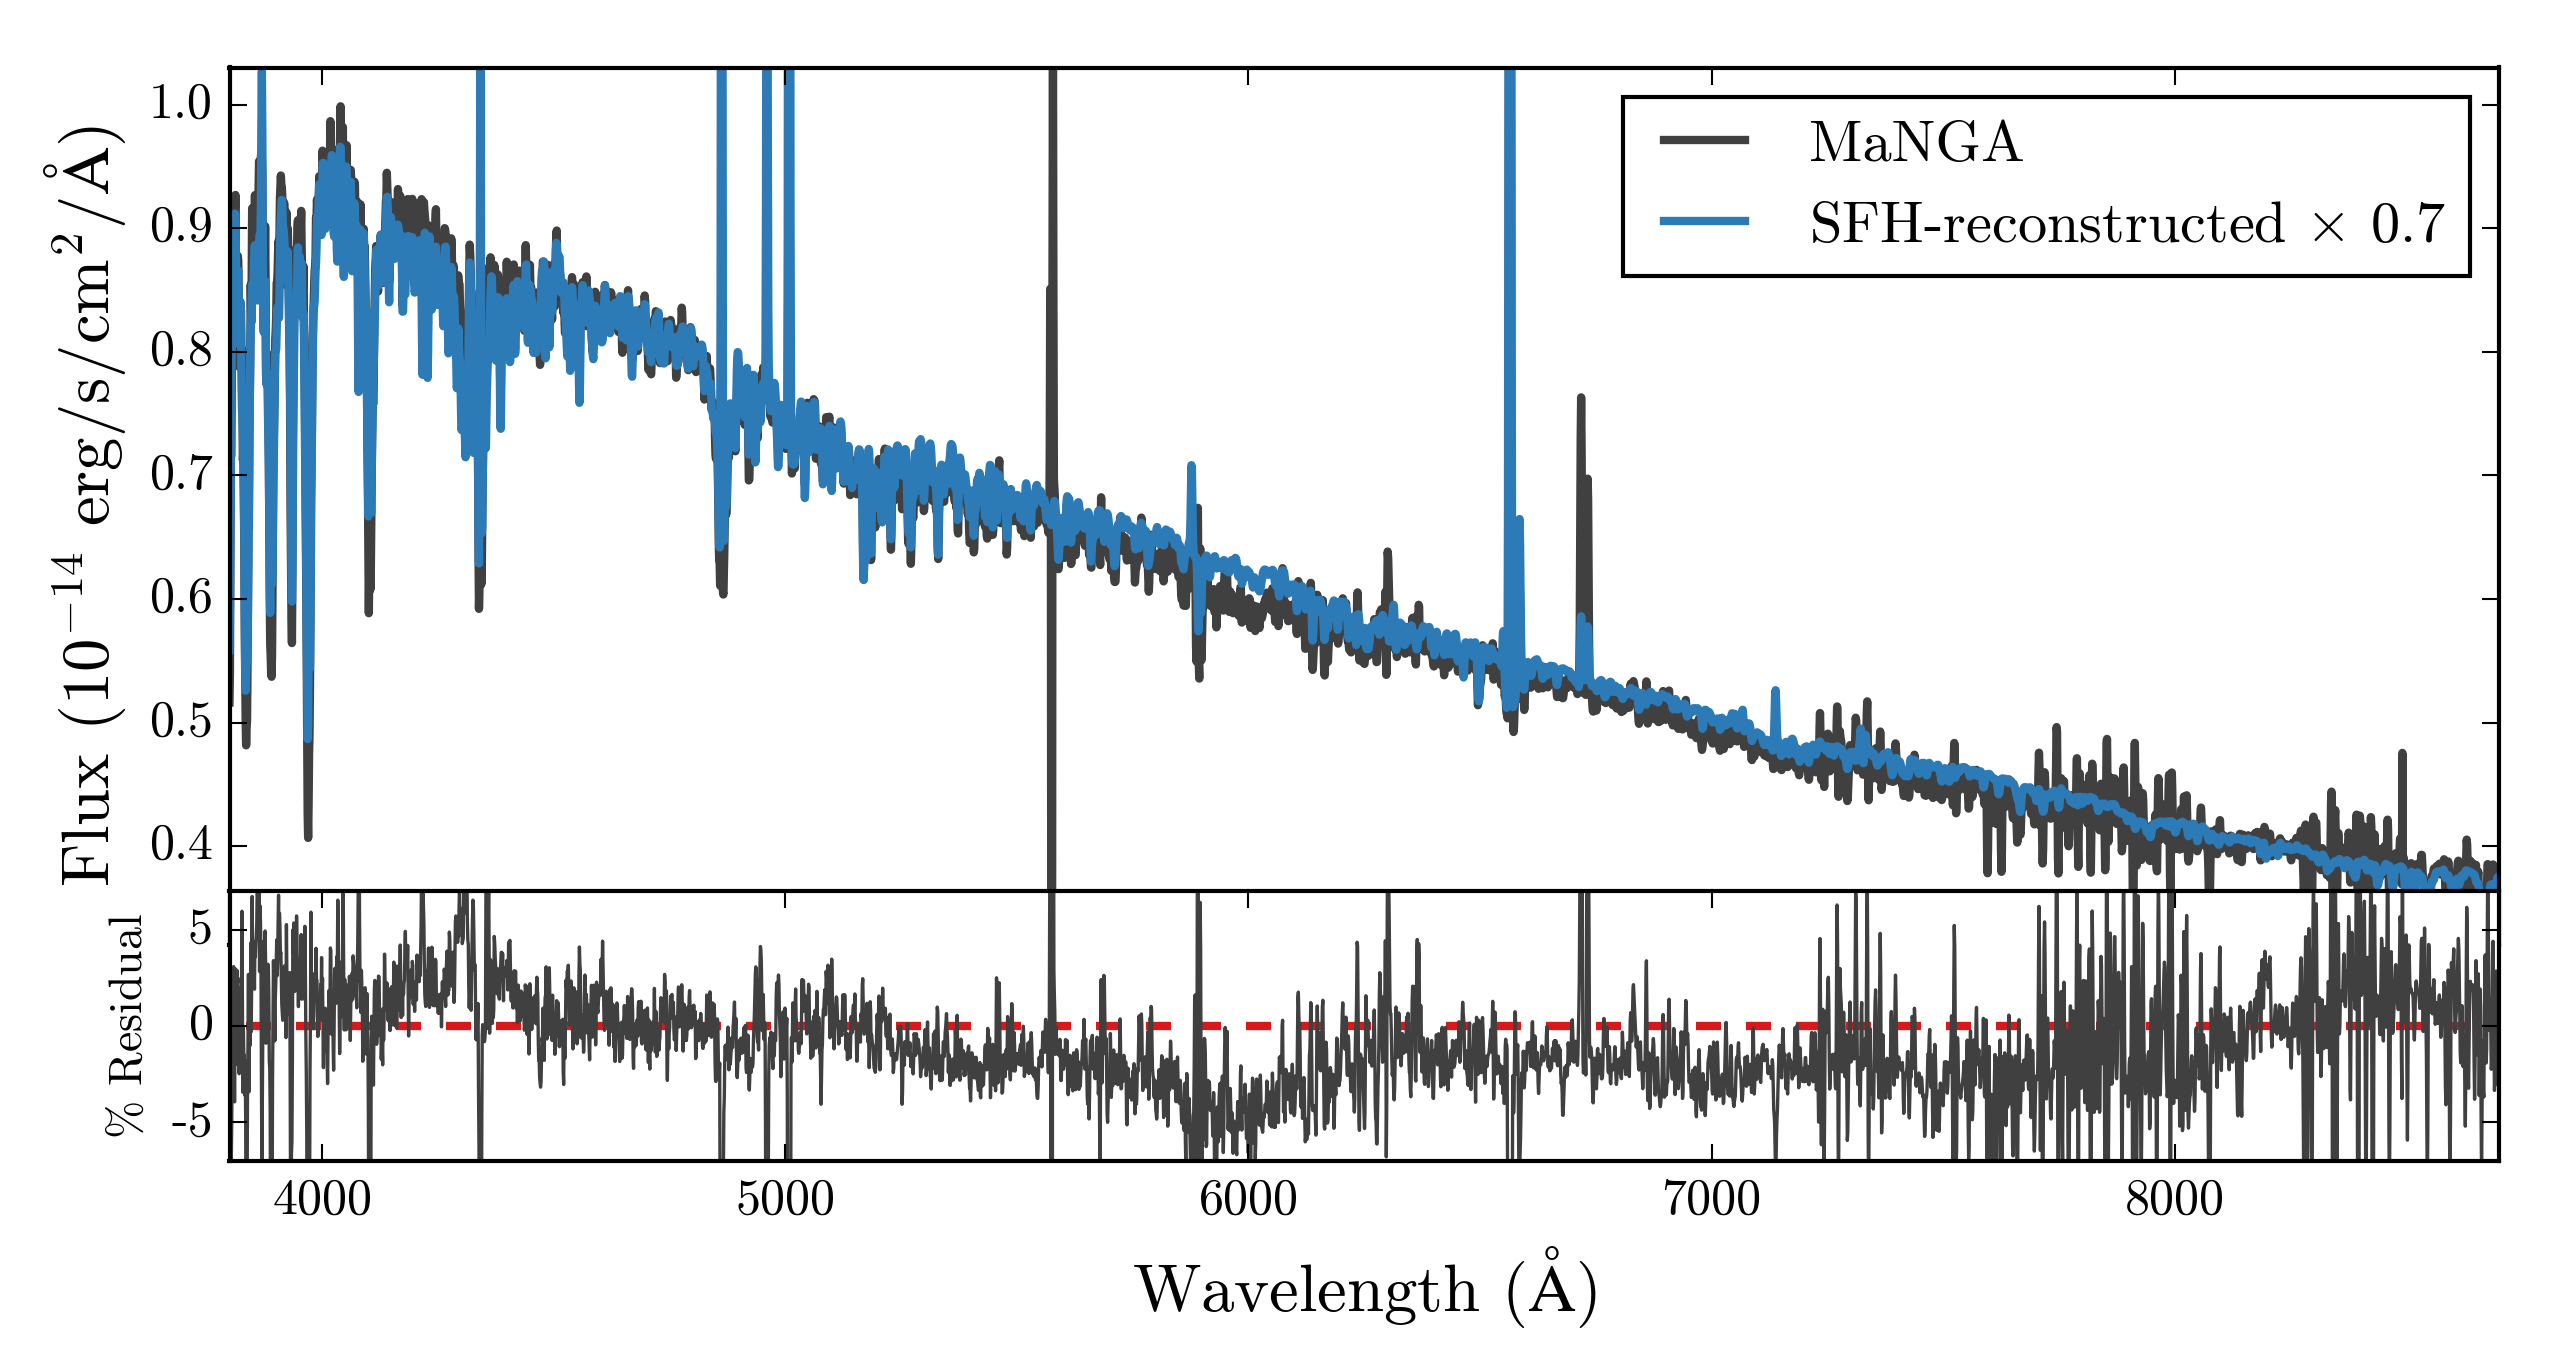
\includegraphics[width=\linewidth]{figs/f6.png}
    \caption{{\sc Comparing the total summed MaNGA spectrum with the spectrum synthesized from the CMD-inferred properties---} The total summed MaNGA spectrum (black), from 3800 to 8800\ang, compared with the model spectrum reconstructed from the CMD-inferred SFH, CEH, and reddening (blue). The bottom panel shows the percent residual error between the observed spectrum and the synthetic spectrum. There is good overall agreement between the data and model spectra, with deviations less than 5\% over the full wavelength range considered. However, we note that the synthesized spectrum has been scaled down by 70\% to match the observed flux level, likely a repercussion of the shallow photometry.}
    \label{fig:fullSpec}
  \end{center}
\end{figure*}
%-------------------------------------------------------

%-------------------------------------------------------
% Figure 6: spectra sub-plots
%-------------------------------------------------------
\begin{figure*}
  \begin{center}
    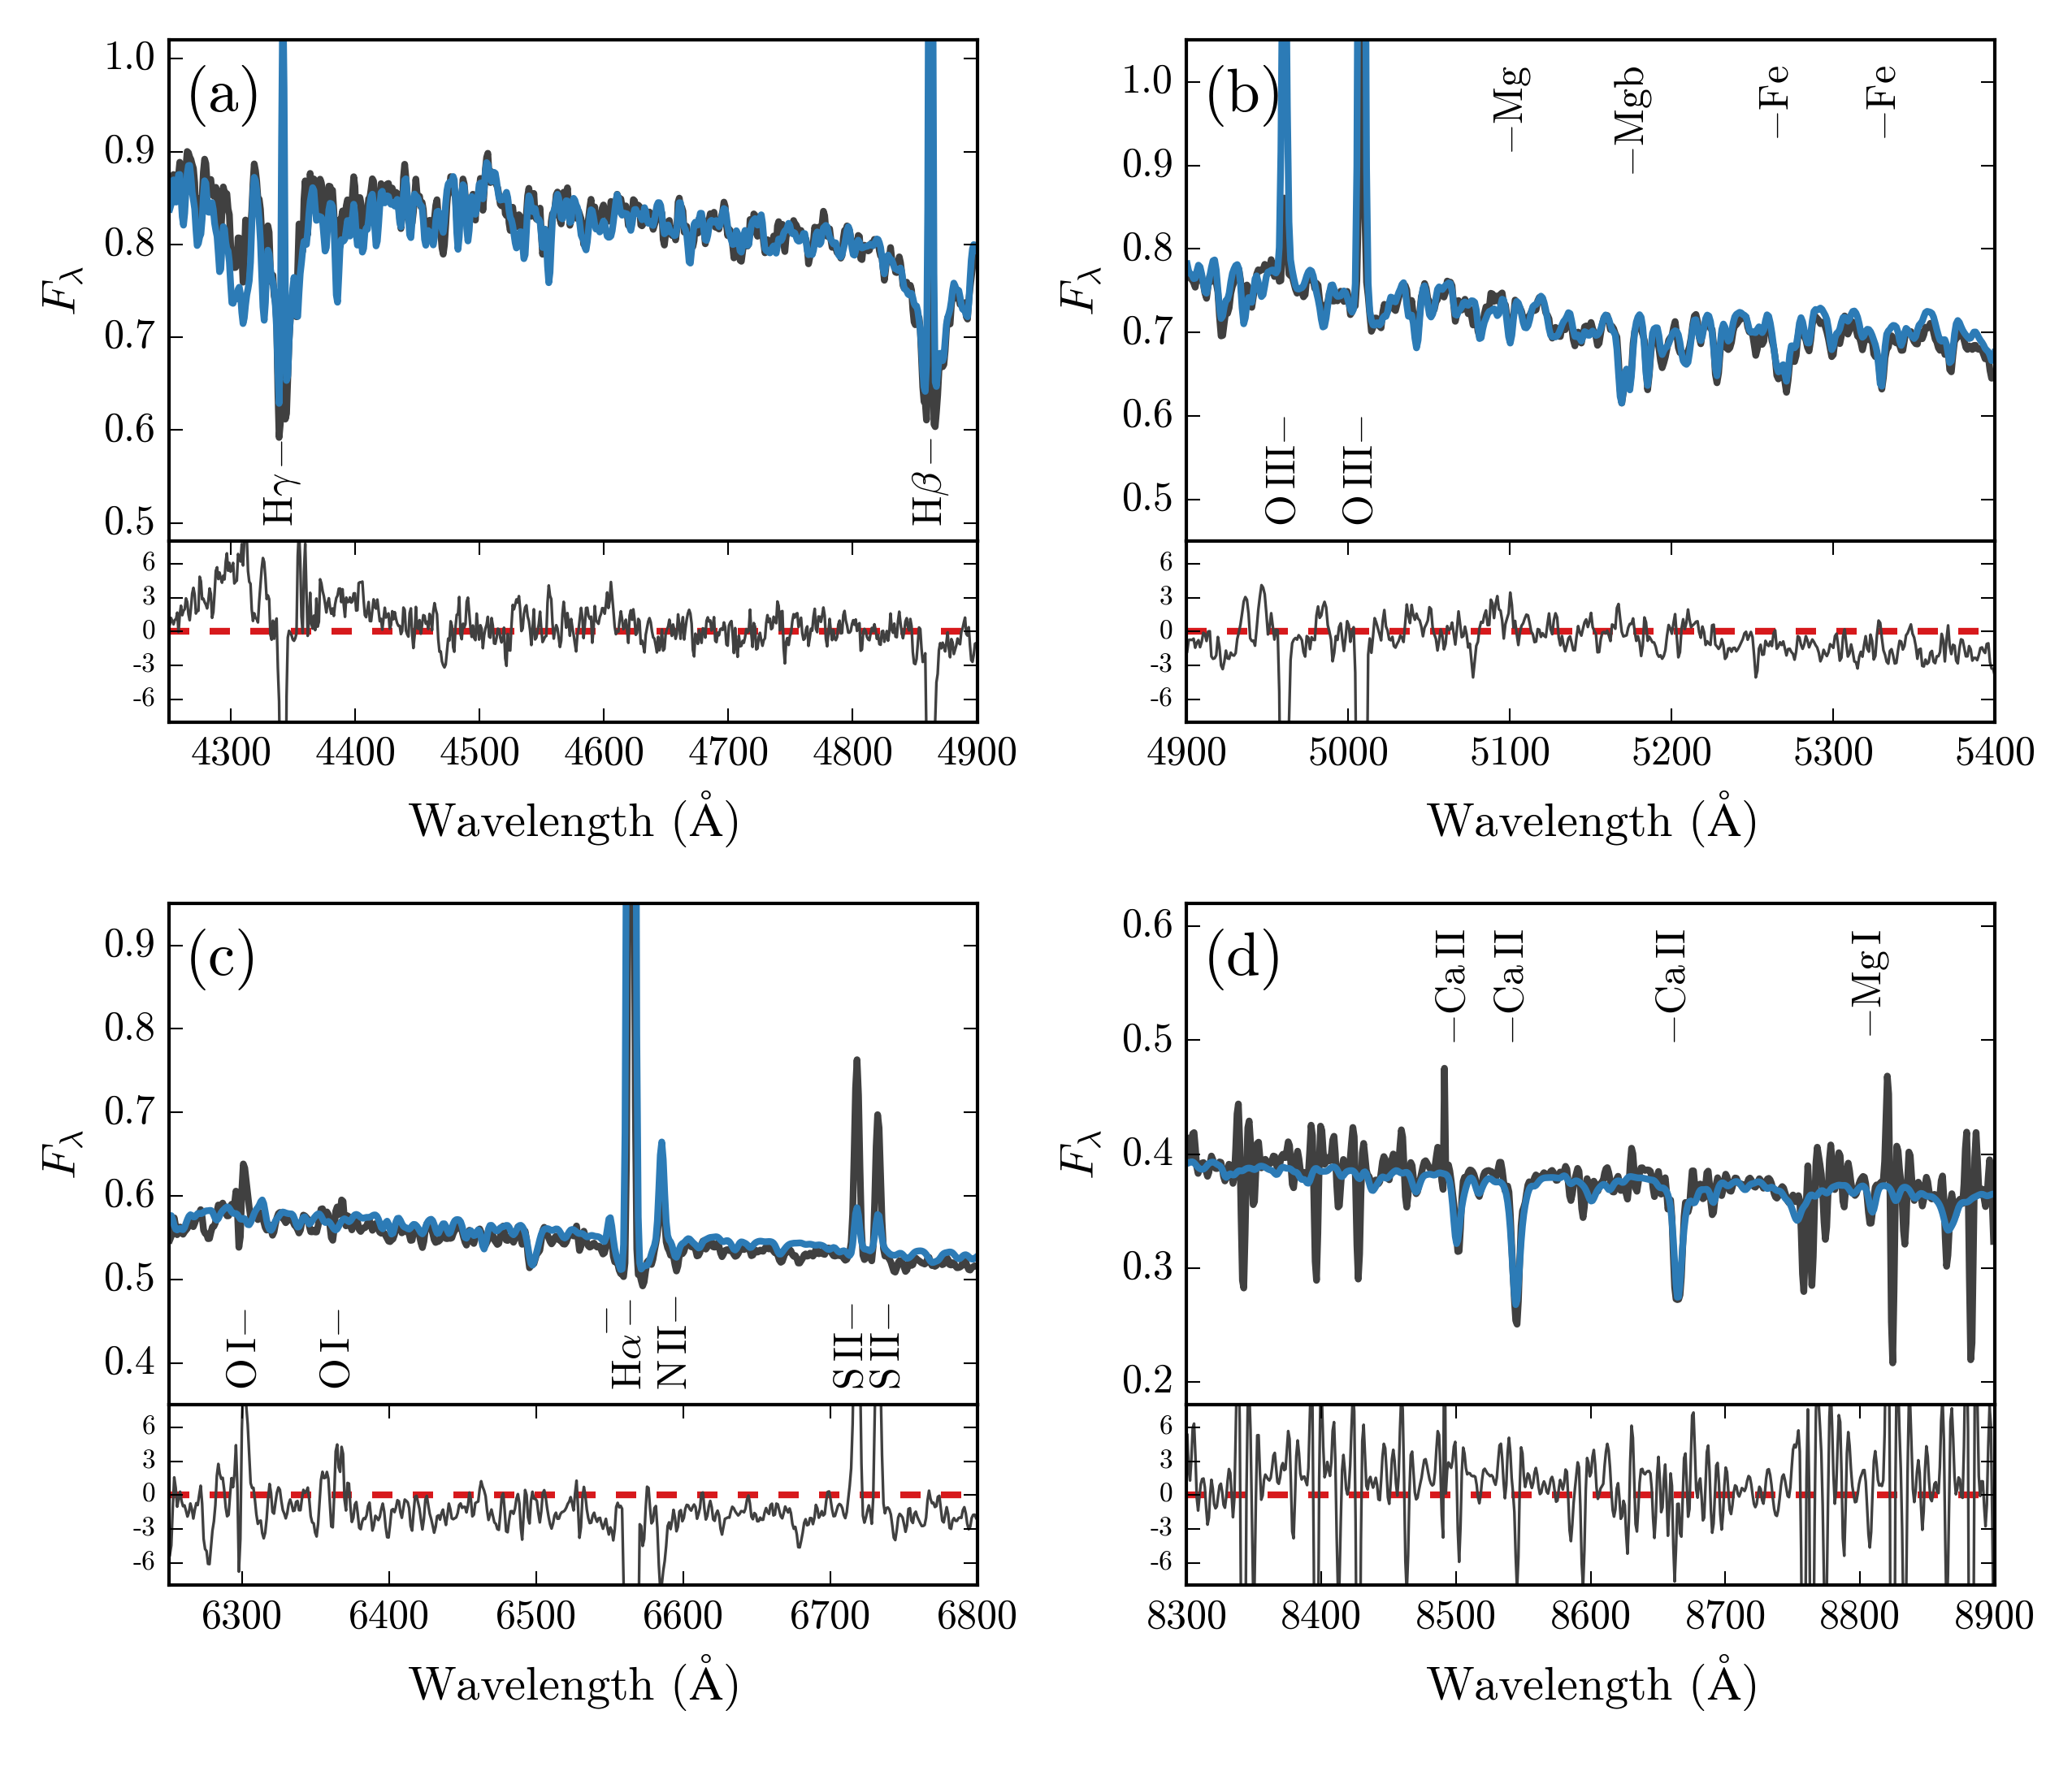
\includegraphics[width=\linewidth]{figs/f7.png}
    \caption{{\sc A detailed comparison of spectral features for the total summed MaNGA spectrum and the CMD-synthesized model spectrum---} The total summed MaNGA spectrum (black) is compared to the model spectrum synthesized from the CMD-inferred properties (blue). In each panel, the model spectrum has been multiplied by 0.7 and the percent residuals are shown below the spectrum, with the red dashed line indicating 0\%. After correcting for the bulk flux offset, the model deviates from the observed spectrum at the 5\% level, remarkable agreement considering that there has been no fine-tuning of the CMD-inferred properties.}
    \label{fig:zoomSpec}
  \end{center}
\end{figure*}
%-------------------------------------------------------
%{\bf (a)}: The spectrum from 4200 to 4900\ang, which covers the H$\gamma$ and H$\beta$ lines. Absorption features are well matched in shape, but the SFH-reconstructed spectrum is too red and shows a bulk offset from the observed spectrum.
%{\bf (b)}: The spectrum from 4900 to 5400\ang covers two nebular emission lines (\oiii$\lambda$\,4959 and \oiii$\lambda$\,5007) and magnesium and iron absorption features. The strength of the Mg lines are often used as a stellar metallicity anchor, and it is encouraging that the synthesized spectrum agrees well with the observed spectrum here, despite the overall flux offset.
%{\bf (c)}: The wavelength range from 6200 to 6800\ang covers several nebular emission lines, including \nii$\lambda$\,6548,6584, \ha, and \sii$\lambda$\,6719, 6731. \sii is significantly detected in the observed spectrum, but not predicted in the model spectrum.
%{\bf (d)}: The spectrum from 8300 to 9000\ang covers the calcium triplet, which is a frequently used metallicity diagnostic. The synthesized spectrum agrees well with the observed spectrum here, highlighting the consistency between the CMD-inferred metallicity and integrated light techniques.
\subsection{Spectral Fitting with Prospector}\label{sec:results:pros}

The top panel of Figure~\ref{fig:prospector_spec} compares our maximum a posteriori (MAP) \texttt{Prospector} model (blue) to the observed MaNGA spectrum of NGC 4163 (black). Missing regions from the model spectrum were masked during the fitting process; only the continuum was fit between $4000-7000\,\mathrm{\AA}$, with nebular emission lines excluded. The bottom panel shows the residuals (i.e., observed / model spectrum) as a function of wavelength. The quality of this fit is similar to that of the FSPS-reconstructed spectrum shown in Figure~\ref{fig:fullSpec}: the residuals are $\leq$5\%, and show a similar coherent structure near $6000\,\mathrm{\AA}$. However, there is more structure in the residuals of the \texttt{Prospector} fit than for the detailed reconstruction; this somewhat poorer fit is expected, as the SFH, metallicity, and dust models are all much simpler here.

\begin{figure*}[!ht]
\begin{centering}
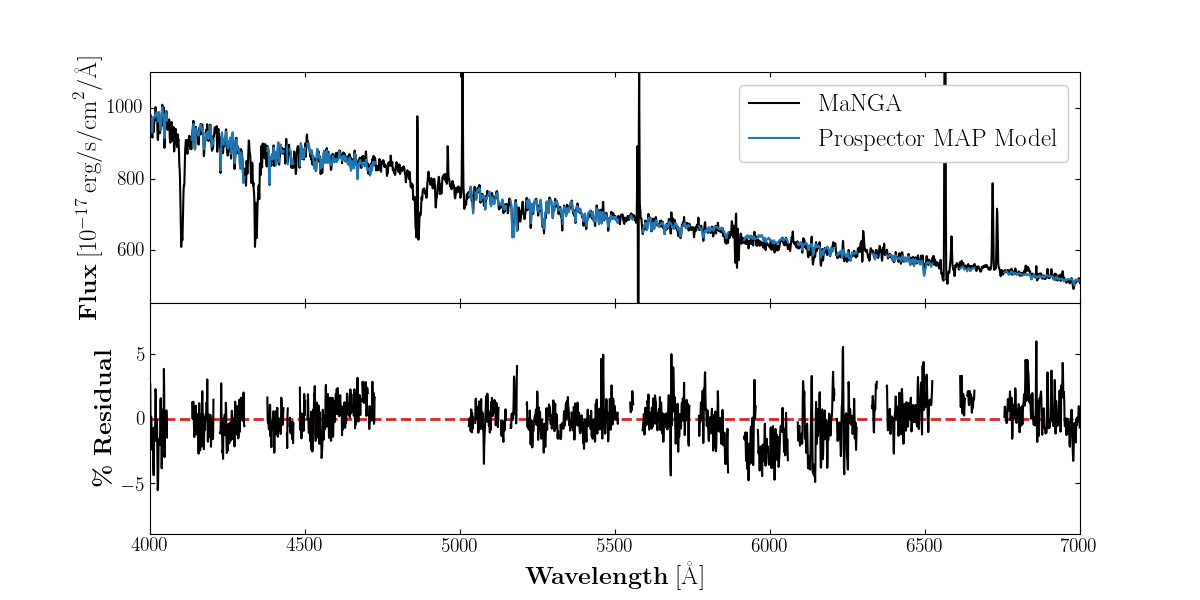
\includegraphics[width=\linewidth]{figs/prospector-spec-resid.png}
\caption{{\sc The best-fit Prospector model to the NGC 4163 MaNGA spectrum.} Top: the maximum a posteriori (MAP) \texttt{Prospector} model (blue) is overplotted on the observed MaNGA spectrum (black). Gaps in the model spectrum are regions that were masked in the fit; only the continuum was used. Bottom: residuals (model / observed spectrum) of the MAP \texttt{Prospector} model. The agreement is generally good, with $\lesssim5\%$ residuals, though there is some coherent structure around 6000 $\mathrm{\AA}$ and toward redder wavelengths. \label{fig:prospector_spec}}
\end{centering}
\end{figure*}

\begin{figure}[!ht]
\begin{centering}
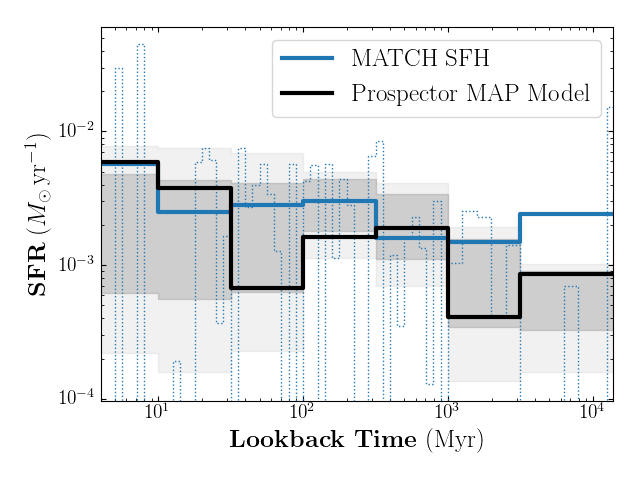
\includegraphics[width=\linewidth]{figs/prospector-sfh.png}
\caption{{\sc Comparison of SFHs derived from CMD-fitting and spectral fitting.} The best fit SFH for NGC 4163 from MATCH is shown in blue, while the dotted blue line shows the SFH at the native MATCH resolution. The black line shows the maximum a posteriori model from Prospector, and the light and dark grey shaded regions show the 5-95 and 16-84 confidence intervals, respectively, of the PDFs in each age bin. Overall, there is remarkably good agreement between the shape of the MATCH SFH and the \texttt{Prospector} SFH PDFs, especially at recent ages. However, at the oldest ages, MATCH infers a higher SFR and therefore a higher total stellar mass formed than \texttt{Prospector}. \label{fig:prospector_sfh}}
\end{centering}
\end{figure}

Figure~\ref{fig:prospector_sfh} compares the SFR as a function of age (or lookback time, shown on a logarithmic scale) inferred from CMD modeling with MATCH to that inferred from spectral fitting with \texttt{Prospector}. The \texttt{Prospector} maximum a posteriori (MAP) SFH is shown as the solid black line, with the light and dark grey shaded regions showing the 5-95 percentile and 16-84 percentile ranges of the posterior distribution. The MATCH SFH is shown at native resolution as the blue dotted line, and rebinned to the time resolution of the \texttt{Prospector} model as the solid blue line.

Overall, these two SFHs agree remarkably well, given that they were inferred using different data \textit{and} different modeling techniques. The shapes of the SFHs are very similar, particularly when comparing the MATCH SFH to the 16-84 percentile range of the \texttt{Prospector} PDFs; note that the MAP model is just one sample, and does not fall in the center of the posteriors in every age bin. Indeed, in every age bin except the oldest (ages $\geq 3$ Gyr), the MATCH model agrees well with the \texttt{Prospector} fit. The only major discrepancy is the SFR in the oldest age bin, and therefore the total stellar mass formed; we discuss this mismatch in Section~\ref{sec:mass_offset} below.


\section{Discussion}\label{sec:discussion}

\subsection{Stellar Mass in MATCH vs. FSPS}
\label{sec:mass_offset}

As seen in Fig.~\ref{fig:prospector_sfh} above, there is a mismatch between the total stellar mass formed (also the total luminosity of the galaxy) between the SFHs inferred using MATCH vs. \texttt{Prospector}. The MAP FSPS model has a stellar mass of $\log{M_\star/M_\odot} = 7.1$, vs. the MATCH value of $\log{M_\star/M_\odot} = 7.5$. The FSPS model has $0.4\times$ the stellar mass inferred by MATCH, a worse mismatch than the factor 0.66 normalization offset between the observed and model spectra. This difference could easily be attributed to the different spectral library, isochrone set, and/or dust model adopted in the \texttt{Prospector} model.

\todo{The following is my best, current understanding of some of the drivers of mass/luminosity offsets between MATCH and FSPS...}

There are several factors that result in stellar masses from MATCH and FSPS not being directly comparable:
\begin{enumerate}
\item \textit{Low-mass IMF cutoff} -- MATCH does not impose a lower mass cutoff on the IMF, essentially resulting in a more bottom-heavy IMF than used in FSPS. Since the higher-mass stars that are detectable in observed CMDs are used to infer the presence of low-mass stars below the detection limit, this difference in ``effective'' IMF makes MATCH-based $M_\star$ systematically higher than FSPS (which imposes a low-mass cutoff of $0.1 \,M_\odot$, by a factor of 1.2 for a \citet{kroupa01} IMF. 
\item \textit{Binary Fraction} -- A binary fraction ($f_\mathrm{binary}$) is adopted in MATCH to handle the presence of blended binary stars in the CMD. If the binary fraction were set to 0, the MATCH model would be biased by the presence of ``single'' stars that are too bright for their colors; by contrast, SPS models are not affected by this issue because they only model the total, unresolved light from stellar populations. MATCH assumes that binary companions have a stellar mass drawn from a uniform distribution: [0, $m_\mathrm{primary}$], where $m_\mathrm{primary}$ is the companion star's mass. An underappreciated effect of this binary fraction implementation in MATCH is that the total stellar mass formed is increased by a factor of $1 + f_\mathrm{binary} / 2$. For $f_\mathrm{binary}=0.35$, as used in the MATCH model in this work, the MATCH mass boosted by a factor of 1.175 relative to what would be appropriate for a FSPS model.
\item \textit{Foreground contamination} -- MATCH requires a model of expected contamination by foreground stars to properly account for the presence of stars in unexpected regions of the CMD. If the foreground model is not adequate to fully account for contamination in the CMD, then such contamination can lead MATCH to infer the presence of excess low-mass stars below the detection limit. This effect is harder to quantify, but could easily cause an upward bias in stellar mass at the level of $\sim10-20\%$.
\end{enumerate}

\subsection{Flux offset}\label{sec:discussion:offset}

After the total stellar mass from MATCH is adjusted to the scale appropriate for FSPS use ($1/1.175 = 0.85$), the SFH-reconstructed spectrum is still brighter than the total observed spectrum by 10-15\%. In what follows, we highlight additional sources of error that could drive such an offset. None of these alone is responsible for the total offset, however, we suggest that the combination of several could easily explain a 10-15\% flux offset.

\paragraph{Missing flux in the MaNGA summed spectrum} As described in \S\ref{sec:data:manga}, we use the MaNGA pixel mask to remove spaxels marked as unacceptable for science from the total summed spectrum. In the aperture-matched region, roughly 6\% of the 3266 spaxels ($N=200$) are flagged by the pixel mask. These masked spaxels are located at the outer edges of the IFU, and contribute less than $5-7$\% of the total flux. 

\paragraph{Stellar models} the hybridMC errors calculated for the MATCH SFH give an estimate of the uncertainties driven by temporal stochasticity in star formation. They do not, however, account for systematic uncertainties driven by the use of particular isochrone sets, which we test here. To do this, we run MATCH on the photometry matched to the MaNGA footprint with identical parameters, using two different isochrone sets: the fiducial Padova isochrones presented in \S\ref{sec:methods:fsps} and the Mesa Isochrones and Stellar Tracks \citep[MIST;][]{Dotter+2016, Choi+2016}, single-star stellar evolutionary models which include the effect of stellar rotation.

In Fig.~\ref{fig:tracks}, we show the best-fit SFHs using Padova (blue) and MIST (orange). The SFHs agree within their respective error envelopes but the best-fit SFHs show a few major discrepancies. The MIST model predicts a slightly lower SFR in the youngest time bin (0-10\Myr), 0.0048\Msun/yr compared to the 0.0054\Msun/yr in the Padova model. However, the MIST model predicts a much higher SFR in the second-youngest time bin (10-30\Myr), 0.0057\Msun/yr compared to 0.0024\Msun/yr. This suggests that our uncertainties are likely underestimated for populations with ages younger than 30\Myr. These young stars dominate the total luminosity, which can easily account for 10\% variations in flux. \todo{run HMC for MIST}

%-------------------------------------------------------
% Figure B: Spectrum [4900-5400]
%-------------------------------------------------------
\begin{figure}
  \begin{center}
    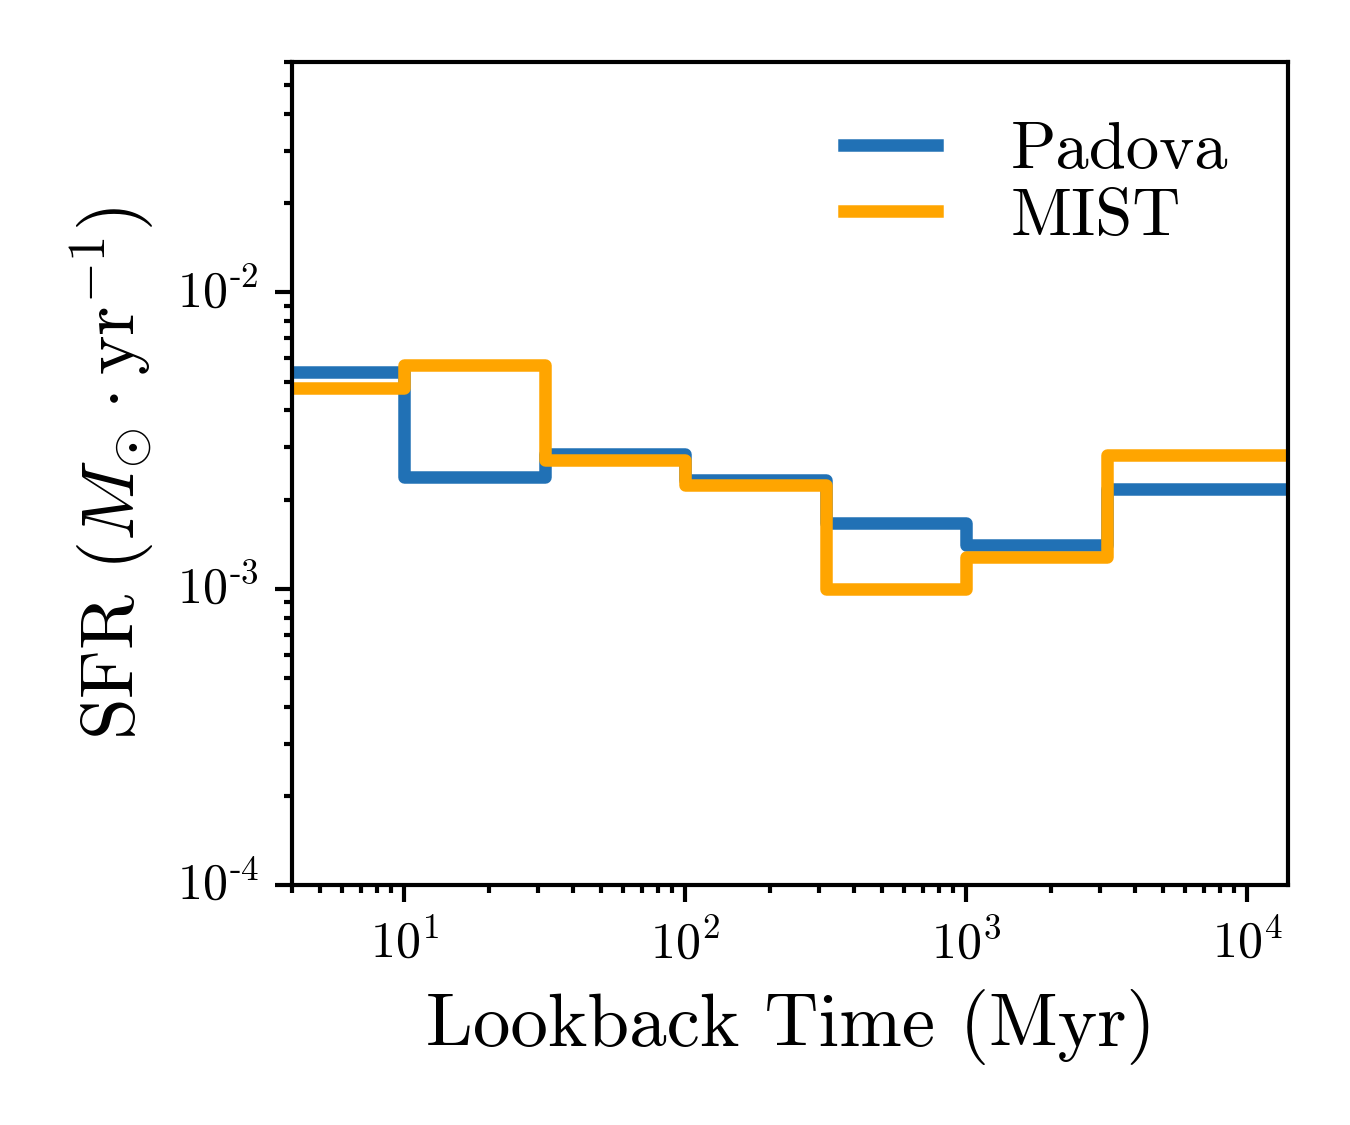
\includegraphics[width=\linewidth]{figs/tracks_SFH_comp.png}
    \caption{{\sc Best-fit SFHs from CMD-fitting using different stellar models---} Placeholder for figure comparing MIST and Padova.}
    \label{fig:tracks}
  \end{center}
\end{figure}
%-------------------------------------------------------

\paragraph{Spatial variation in differential reddening and photometric completeness} The MaNGA observations target the crowded center of NGC 4163, where the photometric completeness shows significant spatial variation. In particular, there is a star-forming knot near the center of the MaNGA FoV, where the high stellar density paired with several very bright stars produce much lower levels of photometric completeness. To assess the degree that varying photometric completeness has on our SFH recovery, we use MATCH to measure SFHs on a region-by-region basis. \todo{Need to re-run these so that I can compare them in a consistent way with current best-fits}
%Due to the non-negligible degree of varying completeness, we may want to measure SFHs on a region-by-region basis, and then combine them as necessary. Initial tests of subregion comparisons have proven to be highly sensitive to spatial variations in differential reddening found in the various star forming knots.

\section{Conclusions}\label{sec:conclusions}

In this work, we have presented a detailed comparison of properties derived with SED fitting and CMD fitting for the nearby dwarf galaxy NGC 4163. Our conclusions are as follows:

\begin{itemize}
    \item Using the CMD-fitting code MATCH, we have derived the star formation history, chemical enrichment history, and the dust content for the stars in the region mapped to the MaNGA IFU observations (\S\ref{sec:results:match}).
    \item We reconstruct the optical spectrum for the aperture-matched region using the CMD-derived derived SFH, CEH and dust as input to FSPS. Despite an overall offset in flux, the reconstructed model spectrum is in good agreement with the total summed MaNGA spectrum, with similar colors and key spectral features well-matched in shape and depth (of order 3\% residuals; \S\ref{sec:results:fsps}). Notably, absorption features sensitive to metallicity and age show good agreement, highlighting the consistencies between resolved star and integrated light techniques.
    \item We use {\tt Prospector}, a Bayesian spectral fitting code, to infer the SFH from the total summed MaNGA spectrum, using a flexible SFH parameterization analogous to the MATCH time bins. We find remarkably good agreement between the MATCH SFH and the {\tt Prospector} SFH, especially at recent ages (0-10\Myr, 30-100\Myr). However, this agreement worsens for older age bins (4-10\Gyr), where MATCH predicts a higher SFR and thus a higher total stellar mass (\S\ref{sec:results:pros}).
    \item {\tt Prospector} estimates a stellar mass of $\log{M_\star/M_\odot} = 7.1$, compared to the MATCH value of $\log{M_\star/M_\odot} = 7.5$. The {\tt Prospector} stellar mass is 0.4 times the stellar mass inferred by MATCH, a worse mismatch than the 0.7 flux normalization offset between the observed and reconstructed model spectrum. We suggest that the combination of several factor-of-a-few uncertainties can explain the difference in total stellar mass and flux offset. These include: the difference in dust models used in MATCH and {\tt Prospector}; the implementation of binary stars and foreground star contamination in MATCH; the shallow photometric completeness in NGC 4163 and spatial variation in photometric completeness and differential extinction (\S\ref{sec:discussion}). 
\end{itemize}

Ultimately, this study was limited by the relatively shallow photometric depth in the region of NGC 4163 observed with MaNGA. Moreover, in terms of assessing SFH recovery from SED-fitting, it represents a single data point. In future work, we will extend this important exercise to M31, where we have IFU observations targeting regions that span a range in ancient and recent SF, dust column density, dust geometry, and stellar metallicity.


%%%%%%%%%%%%%%%%%%%%%%%%%%%%%%%%%%%%%%%%%%%%%%%%%%%%%%%%%%%%%%%%%%%%%%%%%%%%%%%%
%-------------------------------------------------------
\bibliographystyle{aasjournal}
\bibliography{main}
%-------------------------------------------------------
\end{document}